%%%%%%%%%%%%%%%%%%%%%%%%%%%%%%%%%
%
%このファイルは3回のコンパイルの後,
%同梱の./listofcontents.shを用いて
%./listofcontents.sh ファイル名からドットと拡張子を除いたもの
%を1回実行し,最後にもう一度コンパイルをする必要があります.
%
%また,同梱のkanzawa.sty, kanzawa_m.sty, kanzawa2.sty, moreverb.*,
%listofcontents.sh, here.sty, jtygm.sty,
%も必要になります.
%
%
%%%%%%%%%%%%%%%%%%%%%%%%%%%%%%%%%%%
\documentclass[a4j,12pt,dvipdfmx,oneside]{jsbook}
\usepackage{kanzawa2}
\usepackage{here}
\usepackage{times}
\usepackage{amsmath,amsthm,amssymb}
\theoremstyle{definition}
\newtheorem{theorem}{定理}
\newtheorem*{theorem*}{定理}
\newtheorem{Def}[theorem]{定義}
\newtheorem*{Def*}{定義}
\newtheorem{Alg}[theorem]{アルゴリズム}
\newtheorem*{Alg*}{アルゴリズム}
\usepackage{mathptmx}
\usepackage{pifont}
\usepackage{tascmac}
\usepackage{oldgerm}
\usepackage{jtygm}
\usepackage{type1cm}
\setlength{\textwidth}{\fullwidth}
\newcommand{\vd}{\mbox{d}}
\def\rthree{I\kern-2ptI\kern-2ptI}
\newcommand{\namelistlabel}[1]{\mbox{#1}\hfil}
\newenvironment{namelist}[1]{
	\begin{list}{}
		{\let\makelabel\namelistlabel
		\settowidth{\labelwidth}{#1}
		\setlength{\leftmargin}{1.1\labelwidth}}
}{
\end{list}}

\usepackage[T1]{fontenc}
\usepackage{textcomp}
\usepackage[utf8]{inputenc}
\usepackage{lmodern}
\usepackage[all, warning]{onlyamsmath}
\kanjiencoding{JY1}
\kanjifamily{mc}
\kanjiseries{m}
\kanjishape{n}
\selectfont
\usepackage{enumitem}
\newcommand{\argmax}{\operatornamewithlimits{\mathrm{arg\,max}}}
\newcommand{\argmin}{\operatornamewithlimits{\mathrm{arg\,min}}}
\newcommand{\QED}{\hfill$\blacksquare$\par}
\usepackage{longtable}
\usepackage[dvipdfmx]{graphicx}
\usepackage{mediabb}
\makeatletter
\def\minimize{\mathop{\operator@font minimize}} 
\makeatother
\usepackage{eclbkbox}	% required for `\breakbox' (yatex added)
\begin{document}
\pagestyle{headings}
\def\thepage{\roman{page}}
\input epsf
\tableofcontents
\listoffigures
\listoftables
%%%%%
\newpage
\pagestyle{myheadings}
%
%
%
\chapter{序論}
\def\thepage{\arabic{page}}
\setcounter{page}{1}
\label{chap:first}
%
%
%
\section{背景}\label{sec:background}
%
%
%
\subsection{\LaTeX}\label{subsec:latex}
%
%
%
「\LaTeX{}はとっつきにくいけど,凄い」っていう文章が
ここに入っていると思って下さい.
でも,
「\LaTeX{}は凄いけど,とっつきにくい」
のも一理ある.
っていう内容の,
エレガントな文章がここに入っていると思って下さい.
%
%
%
\subsection{学術文書としての卒業論文}\label{subsec:academic_statement}
%
%
%
理工学系論文特有の書き方っていうのがあって,
当研究室の卒業論文はその一種なんだけど,
卒業論文を書く皆さんは,そんな理工学系論文を初めて書くわけで,
色々面倒臭い決まりがいっぱいある.
っていう内容の,エレガントな文章がここに入っていると思って下さい.
%
%
%
\subsection{当研究室固有の決まりごと}
%
%
%
卒業論文を作成するっていうのは,そりゃもう大変な作業な訳で,
ただでさえ色々注意しなきゃいけないことがあるのに,
うちの研究室で卒論書くからにはこれは守ってもらわなきゃ困るっていう
ローカルルールもある.
って,その必要性を問われると,
公正な回答をする自信が今一つないのだけど,
まぁ,この研究室に配属されたのだから
我慢するしかない.
っていう内容の理路整然とした文章がここに入っていると思って下さい.
%
%
%
\section{目的}\label{sec:purpose}
%
%
%
本文書は,
当研究室で,卒業論文を作成するにあたって,注意すべき事項を記したものです.
ただし,過去の卒業研究において運用されていた内容がそのまま記載されていた
り,
今年度の卒業研究において大変重要な注意事項が盛り込まれていなかったり
など,
現状を反映していない部分もあるので,
疑問があれば必ず,指導教員に確認して下さい.
%
%
%
\section{構成}\label{sec:contents}
%
%
%
本文書の構成を次に示します.
第\ref{chap:checkManuscript}章では,指導教員に原稿を校正させることについて
説明しています.
第\ref{chap:abst}章では,卒業論文概要書作成について
説明しています.
第\ref{chap:thesis}章では,卒業論文作成について
説明しています.
第\ref{chap:presen}章では,発表資料作成について
説明しています.
第\ref{chap:statement}章では,卒業論文概要書,卒業論文,および発表資料に盛
り込まれる文章について
説明しています.
第\ref{chap:math}章では,卒業論文概要書,卒業論文,および発表資料に盛
り込まれる数式について
説明しています.
第\ref{chap:experiment}章では,卒業論文概要書,卒業論文,および発表資料に盛
り込まれる数値実験について
説明しています.
第\ref{chap:cite}章では,卒業論文概要書,および卒業論文に盛
り込まれる参考文献について
説明しています.
第\ref{chap:reference}章では,\LaTeX{}を用いて卒業論文概要書や卒業論文を作
成する際の参照機能を説明しています.
第\ref{chap:latex-rule}章では,その他の\LaTeX{}のルールを説明しています.
第\ref{chap:multimedia}章では,\LaTeX{}における図表とプログラムソースの取
り扱いについて説明しています.
最後に第\ref{chap:conclusion}章では,本文書の結論を述べています.
また,付録では,
原稿チェックリスト,過去の卒業研究中間発表会と卒業研究発表における配布資
料を掲載してます.
%
%
%
\section{注意}
卒業論文をはじめ,卒業論文概要書や卒業研究発表資料を作成するに当たって,
指導教員からの直接の指導とは別に,多くの研究者による論文・書籍,
過去の卒業論文を参考にすると思います.
また,大いに参考にして欲しいと思います.
しかし,書き方についてそれらを鵜呑みにしてはいけません.

論文・書籍の文章は,著者の癖に著しく依存し,
内容が素晴らしいからといって,
その文章が素晴らしいとは限りません.
また,著名な先生の文章はあまりにエレガントすぎて,
それを猿真似すると,そこだけ浮きます.
必ず,自分の脳で消化し,自分の文章で書いて下さい.
結果として同じ字面になるのならばそれはそれで結構です.
一方で記法は,
研究閥や著者の思想,
さらに言えば同じ著者でもその文書の思想によって大きく異なる可能性がありますので,
偉い先生の書いた本の定義や定理をそのまま写しても,
指導教員に改訂を要求されることがあります.

また,過去の卒業論文を参考にする際,
「どの程度が合格ラインなのか」という視点で参考にしないで下さい.
参考にしようとしている卒業論文は,指導教員が良しとしたものではないかも知れませんし,
また,そのような視点で過去の卒業論文を参考にして自分の卒業論文を作成すると,
概して,参考にした卒業論文のレベルを下回るからです.
%
%
%
\chapter{原稿を指導教員に校正させるとき}\label{chap:checkManuscript}
%
%
%
\section{はじめに}\label{sec:checkManuscript_intro}
本章では,卒業論文概要書や卒業論文などの作成した文書を指導教員に校正させ
る上での注意点が書かれています.
まず第~\ref{sec:checkManuscript_abst}節でその概要を示し,
次に第~\ref{sec:checkManuscript_misc}節でその他の注意点を示しています.
%
%
%
\section{概要}\label{sec:checkManuscript_abst}
理想的には,原稿に流れ図を添付し,
流れ図中の各項目と原稿の文章の各部の対応を明記した上で,
本文書添付付録のチェックリスト頁をコピーし,
チェックリストの全項目をチェックし,
確認欄にチェックサインの上,原稿に添付するのが望ましいのですが,
これが理想であることを踏まえて現実的に対応して下さい.

自分の原稿を音読し,意味の通らない個所,流れが止まる個所がないかどうかに
十分注意を払って下さい.
文章を少し変更することによって論文全体を変更することになるのは
常です.これを厭んで論文を書くことはできません.
盗作厳禁です.盗作ってのは要は他の文書の丸写しってこと.
何かを参考するにしても,必ず理解し,自分なりの文章で書いてください.
助詞の'の'が重ならないように作文して下さい.
章題目・節題目は必要十分の内容にする.
指導教員が口頭で使ったりしている言葉が実は,
正式な用語ではなく,略語だったりスラングだったりする可能性があるので,
それをそのまま活字化してはいけません.

校正に関する全てのメモは卒業研究の単位を取得するまで保管しておいて下さい.
万が一,指導教員が乱心して不正な成績をつけた場合の訴訟資料になります.

校正時に「?」とか「!」と思ったことに関して,
回答を求める場合があります.
次に原稿を提出する際に,回答を用意しておいて下さい.
対面で校正する場合には頭の中に用意しておけばよいですが,
指導教員が校正するときに近くにいない可能性がある場合には,
文書化して下さい.手書きでも印刷でもいいです.

経験上,第一稿から全ての校正を施すことは不可能です.
不足内容の追加・余計な内容の削除・部分の順序の変更など,
概ねの構成が完成されて,新ためて浮彫りになる誤りが多いので,
論文の度重なる改訂を予め覚悟し,残された時間の十分な余裕を持って
第一稿を完成して下さい.

かといって,「どうせ色々直されるのだからテケトーでいいや」
とは絶対に思わないで下さい.
良い論文の作成は,指導教員でなく著者自身の姿勢次第です.
「卒業できるギリギリのレベルの論文ができればいいや」
とは絶対に思わないで下さい.そう思うと,
卒業できないギリギリのレベルの論文になります.
完全にそう思っていることはないでしょうが
(そう思っていたらうちの研究室に配属されたことは本当に本当に不幸です),
一瞬の気の緩みが皆さんを手抜きの深みに導きます.

校正には理由があります.その理由を把握せずに改訂しないで下さい.
理由が分からない場合は必ず,適当な文献を参考にするか質問して下さい.
%
%
%
\section{そのほかの注意}\label{sec:checkManuscript_misc}
提出日前日までに完成させるよう最善の努力をしてください.
さらっと書いてますが,最善の努力とは,最大限の努力です.
「もうこれ以上は絶対にできない」っていう努力です.
「努力すりゃ間に合わなくてもオッケー」じゃないです.
%
%
%
\section{おわりに}\label{sec:checkManuscript_summary}
本章では,卒業論文概要書や卒業論文などの作成した文書を指導教員に校正させ
る上での注意点を述べました.
まず第~\ref{sec:checkManuscript_abst}節でその概要を示し,
次に第~\ref{sec:checkManuscript_misc}節でその他の注意点を示しました.
%
%
%
\chapter{卒業論文概要書作成}\label{chap:abst}
%
%
%
\section{はじめに}\label{sec:abst_intro}
本章では,卒業論文概要書の作成について述べます.
まず第\ref{sec:abst_feature}節で卒業論文概要書の性格を示します.
次に第\ref{sec:abst_flow}節で作業の流れを示します.
最後に第\ref{sec:abst_file}節でサンプルファイルの扱いを示します.
%
%
%
\section{卒業論文概要書の性格}\label{sec:abst_feature}
卒業論文概要書は,本体である卒業論文の要約であり,
それを一読して当該卒業研究の目的と成果が
理解され得なければなりません.
例えば3年生は,
卒業論文概要集を読んで各研究室の卒業研究内容を把握しようとしているようですが,
3年生が皆さんの書いた概要集を読んで,
「神澤研にいきたい!」
って思うかどうかは別にして,
少なくとも,
「神澤研ではこんなことをやってるんだぁ.じゃここにいく事はないね」
と判断がつかなければなりません.
ちなみに,難解な数式を並べたことによって,
「訳分からないからここにいく事はないね」
っていうのはなしです(結論は同じだけど).
勿論,本来,卒業論文概要書は卒業論文の概要という,
卒業論文に付随した公式文書であって,
決して3年生の研究室配属に際しての参考資料のためにあるのではありませんが,
「3年生が分かるように」というのは,
良い目安だと思います.

その一方で,卒業論文概要書はそれ自体で閉じていなくてはならず,
文中の記号や専門用語は当該文書内で定義しなくてはなりません.
決して,「分からなければ本体の卒業論文読んでね」ではダメです.
でも,自分の研究内容を正確に書いていくと,
あっという間に紙面は埋まってしまいます.
もし埋まらなかったら,内容をはしょり過ぎてるってこと.
一度,文章に登場した記号や用語はちゃんと説明しなきゃいけない一方で,
紙面が限られているという制約条件.
実は,卒業論文本体の作成よりも卒業論文概要書作成の方が難しいのです.

そのため,細かい議論は避け,成果を代表する図表を使うことをお勧めします.
当研究室の研究内容は数学的議論が多いため,
定義と定理と数式を書き並べて紙面を埋める卒業論文概要書になりがちですが,
数理の武装で逃げずに,文章で説明するよう努力しましょう.
%
%
%
\section{作業の流れ}\label{sec:abst_flow}
%
%
%
以下に,理想的な作業の流れを示しています.
特に第1, 2, 3小節については,これが理想であることを踏まえて
現実的に対応して下さい.
\subsection{紙面上での定式化}
まず,基となる研究内容を定式化します.
ここで正しくかつ厳密に定式化しておかないと,
後の卒業論文作成・発表資料作成・発表練習時に苦労します.
期限が迫っているからといって,定式化せずに次の作業に移らないでください.
ここで定式化しておけば,後が楽になります.
次の作業が終わる前に指導教員に確認を得て下さい.
%
%
%
\subsection{定式の文章化}
%
%
%
数式などを用いて定式化しておいたものを日本文にしていきます.
一般に,数式を日本文にすることは至難の技ですが,
可能な限り,数式の本質を文章化します.
どうしても日本文にできないものはしかたないので,数式をそのまま使いますが,
どうしても日本文にできない数式のほとんどは研究内容の本質を表すものではなくて
瑣末なものです.つまり「概要」には不要ということになります.
ここで分量や見栄えには拘らないべきです.
内容が定まらないままにこれらに拘り始めると作文の本質を見誤ることになります.
文章作成に関しては第~\ref{chap:statement}章を,
数式に関しては第~\ref{chap:math}章を読み,慎重に校正して下さい.
数値実験に関しては第~\ref{chap:experiment}章を読み,必要事項を明記して下さい.
予め,必要事項を明記できるように実験データをとっておいて下さい.
参考文献は,第~\ref{chap:cite}章を読み,
当文書の参考文献の記述を参考にして下さい.
%
%
%
%
\subsection{紙面上での「構成」の構成}
構成を練ります.
「まえがき」「あとがき」「数値例」「参考文献」は必須です.
「まえがき」と「あとがき」の間に本論が入ることになります.
本論を\ruby{一}{ひと}章にするか,さらに章分けするかは本章の内容に依存しますが,
分量の制約から\ruby{一}{ひと}章にする可能性が高いでしょう.
次の作業が終わる前に指導教員に確認を得て下さい.
%
%
%
\subsection{\LaTeX{}化}
構成を練り終わったら,その構成に基づいて文章を作成します.
まず,
分量やレイアウトに拘らず,
\LaTeX{}を用いて活字化することによる見栄えを気にします.
文章作成に関しては第~\ref{chap:statement}章を,
数式に関しては第~\ref{chap:math}章を読み,慎重に校正して下さい.
次の作業に入る前に指導教員に判断を仰いで下さい.
%
%
\subsection{仕上がりレイアウトや分量の調整}
文字は勿論のこと,図表や数式の全てが印字範囲内に収まっていることを確認し
て下さい.
数式が行幅を超えている場合には,複数行に分けることを検討しましょう.
図が行幅を超えている場合には,図を縮小することになると思いますが,
図内に埋め込まれた文字が,本文中の下付き文字の大きさと同じかそれより大き
いことを確認して下さい.
そうでない場合には作図作業から始めた方がいいかもしれません.
表が行幅を超えている場合に,安直に文字サイズを変更しようとせず,
まずは表レイアウトの妥当性について再度,検討しましょう.
どうしても文字サイズを縮小せざるを得ない場合には
予め指導教員に確認して下さい.
また,本文中の標準文字サイズ(題目の文字サイズや本文中の上付きや下付きで
ない文字のサイズ)を変更しないで下さい.

自分の文書が指定分量に満たない場合には内容が貧弱すぎるので,
もう一度前の作業に戻ります.
指定分量を越える場合には当然,内容を減らさなければなりませんが,
何を減らすかについては指導教員の指示に従って下さい.
ほとんどの場合,単純にある部分を削除することにはなりません.
ここでもう一度,文章や数式を練り直します.
%
%
%
\subsection{提出前の確認}
内容・レイアウト・分量について指導教員から提出許可を得たら,
提出作業に入りますが,ここでもう一度,提出ファイルについて,
全てのフォントが埋め込まれていること,
用紙サイズがA4ポートレートであること,および,
ファイル名が指定にしたがっていることを確認して下さい.
また,締め切り直前に思わぬ事故が発生することもあるため,
提出は期限前に余裕を持つことを心がけて下さい.
%
%
%
\section{ファイル操作}\label{sec:abst_file}
%
%
%
あらかじめサンプルファイル\texttt{sample.tex}とスタイルファイル
\texttt{style.cls}をダウンロードし,
サンプル\LaTeX{}ファイルから,次の通りにPDFファイルを作成します.
\begin{enumerate}
\item 通常通りのコンパイル
\item { }
\begin{center}
\texttt{dvipdfmx -f \~/ipaex.map -d 5 sample.dvi}
\end{center}
によってpdfファイルを得ます.
\item { }
\begin{center}
\texttt{evince sample.pdf}
\end{center}
で印刷仕上がりを確認できます.Alt+Enterで,
用紙サイズがA4であることと,全フォントが埋め込まれていることを確認して下
      さい.
\end{enumerate}
%
%
%
\section{おわりに}\label{sec:abst_summary}
本章では,卒業論文概要書の作成について述べました.
まず第\ref{sec:abst_feature}節で卒業論文概要書の性格を示しました.
次に第\ref{sec:abst_flow}節で作業の流れを示しました.
最後に第\ref{sec:abst_file}節でサンプルファイルの扱いを示しました.
%
%
%
\chapter{卒業論文}\label{chap:thesis}
%
%
%
\section{はじめに}\label{sec:thesis_intro}
本章では,卒業論文の作成について述べます.
まず第\ref{sec:thesis_contents}節で卒業論文の構成を示します.
次に第\ref{sec:thesis_examples}節で卒業論文をより充実したものにするため
の工夫について示します.
最後に第\ref{sec:thesis_file}節でサンプルファイルの扱いを示します.
%
%
%
\section{構成}\label{sec:thesis_contents}
第一章は序論.背景・目的・構成が書かれます.
例えば,第一節を背景・第二節を目的・第三節を構成とします.
さらに細かく分けたいときには「小節」を用います.
背景については図表をカウントしないで2ページ目に及ぶように文章量を稼いで下さい.

ここで,章立てとそのラべリングについて述べておきます.
\LaTeX は参照機能を有しており,それを積極的に用いるべきです.
参照機能は特に,数式や参考文献の参照においてその威力を発揮しますが,
章立てにも参照機能を用いるべきです.\LaTeX における章立は,
\begin{verbatimtab}
\{chapter}{章の名前}
\{section}{節の名前}
\{subsection}{小節の名前}
\end{verbatimtab}
のように行われますが,以下のようにそれぞれにラベルをつけておきます.
\begin{screen}
\begin{verbatimtab}
\{chapter}{章の名前}\label{chap:korekore}
\{section}{節の名前}\label{sec:kakukaku}
\{subsection}{小節の名前}\label{subsec:shikajika}
\end{verbatimtab}
\end{screen}
実際,本章には\texttt{sec:thesis\_contents}なるラベルがつけられています.
これによって,章(節,小節)番号を参照するときに,
\begin{screen}
\begin{verbatimtab}
第~\ref{sec:thesis_contents}節においては$\cdots$
\end{verbatimtab}
\end{screen}
とタイプしておくと,
\begin{screen}
第~\ref{sec:thesis_contents}節においては$\cdots$
\end{screen}
と印刷されることになります.
このラべリングと参照は一見面倒に感じますが,
後になって,新しい章をどこかに挿入することによって章番号がずれても
本文中の参照個所を全てチェックしなくても良いという利点があります.
参照個所のミスは見つけにくい一方で,読者にとっては真に腹立たしいミスであり,
絶対避けるべきであるため,この参照機能使用を義務とします.
尚,上の例ではラベル名を,
\texttt{chap:korekore}のように「章コマンドの略称:名前」のようにしています.
一般には第一文字が英字で以後は英数字,ハイフン`\texttt{-}', アンダーバー`\texttt{\_}'であれば良い
(厳密には他の文字も許されるかも知れないが運用上はないと言って良い)のですが,
ラベル名が重複してはいけないことと,
参照時に何を参照しているかを容易に思い出せるようにするために,
上例のような命名を勧めます.
第~\ref{chap:reference}章も読んで下さい.

第二章以降は準備.題目は各章の内容に従います.
ここで,記号・方法の定義を行います.アルゴリズムは,
\begin{verbatimtab}
\begin{Alg}[題目]
アルゴリズムの内容
\end{Def}
\end{verbatimtab}
のように書きます.
その他,定義・定理・例・補題も同様の形式とします.
それぞれの,書式は同梱の\texttt{kanzawa.sty}を参照して下さい.
これらを「環境」といいます.「環境」の前に,その「環境」の説明を述べます.
例えば,
\begin{screen}
標準的ファジィ$c$-平均法~(Standard Fuzzy $c$-Means: sFCM)は,
次のアルゴリズムにしたがう:
\begin{Alg}[sFCM]~\cite{kanzawa}
\begin{enumerate}[label=\textsc{Step}~\arabic*., labelindent=\parindent, leftmargin=*]
\item
ファジィ化パラメータ$m>1$を設定し,
初期クラスタ中心$\{v_i\}_{i=1}^C$を設定する.
\label{sFCM:enum:initialize}
\item
オブジェクト-クラスタ間非類似度$\{d_{i,k}\}_{(i,k)=(1,1)}^{(C,N)}$を
次のように設定する:
\begin{align}
d_{i,k}=\|x_k-v_k\|_2^2.
\end{align}
\label{sFCM:enum:dissimilarities}
\item
帰属度$\{u_{i,k}\}_{(i,k)=(1,1)}^{(C,N)}$を次のように設定する:
\begin{align}
u_{i,k}=
\frac{1}{\sum_{j=1}^C\left(\frac{d_{i,k}}{d_{j,k}}\right)^{1/(m-1)}}
\end{align}
\label{sFCM:enum:membership}
\item
クラスタ中心$\{v_i\}_{i=1}^C$を次のように設定する:
\begin{align}
 v_i=\frac{\sum_{k=1}^N{}(u_{i,k})^m{}x_k}{\sum_{k=1}^N{}(u_{i,k})^m}.
\end{align}
\label{sFCM:enum:centers}
\item
$(u,v)$が収束すれば終了,そうなければ\ref{sFCM:enum:dissimilarities}へ.\QED
\end{enumerate}
\end{Alg}
本アルゴリズムでは初期設定としてクラスタ中心を与えているが,
初期帰属度を設定して,クラスタ中心,オブジェクト-クラスタ間非類似度,帰
 属度の順に設定することもできる.
\end{screen}
の通り.ここで注意すべきは,アルゴリズム全体で大きな文字として解釈し,そ
の終わりが句点「.」の代わりに「$\blacksquare$」が使われていること.そして,
次に続く文が前のアルゴリズムを補足するものであるために改段落せずに続いて
いること.もし,アルゴリズムの後に,異なる内容を記述する場合には,
\LaTeX{}ソース内で空行を設けて,改段落すること.

準備に相当する章を単一とするか複数の章に分けるかについてはその内容に依存します.

第二章以降,結論に相当する章まではすべて,
第一節を「はじめに」,最終節を「おわりに」とし,各節でその章の要約を述べます.

次は主題.題目は内容に従います.
主題に相当する章を単一とするか複数の章に分けるかはその内容に依存します.
ここでは仮に,eFCMが提案手法であると仮定して,その導出からアルゴリズム記載までの例を示します.
\begin{breakbox}
HCMは,帰属度の制約を$\{0,1\}$から$[0,1]$に緩和してもなお,
最適解は$\{0,1\}$のいずれかになる.
これを特異な状態であるとして正則化することを考える.
正則化項を帰属度に関する負のShannonエントロピーとすると次の最適化問題が得られる:
\begin{align}
&\minimize_{u,v}\sum_{i=1}^C\sum_{k=1}^Nu_{i,k}\|x_k-v_i\|_2^2
+\lambda^{-1}\sum_{i=1}^C\sum_{k=1}^Nu_{i,k}\log(u_{i,k})
\label{eq:eFCM-objective}\\
&\text{subject to }\sum_{i=1}^Cu_{i,k}=1.
\label{eq:eFCM-constraint}
\end{align}
ここで,$\lambda>0$は正則化の度合いを調整するためのファジィ化パラメータである.
この最適化問題を解くことによって得られる手法をエントロピー正則化ファジィ$c$-平均法~(entropy-regularized fuzzy $c$-means: eFCM)と呼ぶ.
最適化問題~(\ref{eq:eFCM-objective}), (\ref{eq:eFCM-constraint})に対応するLagrange関数$L_{\mathsf{eFCM}}(u,v,\gamma)$は次のように表される:
\begin{align}
 L_{\mathsf{eFCM}}(u,v,\gamma)=& \sum_{i=1}^C \sum_{k=1}^N 
 u_{i,k} \|x_k-v_i\|_2^2
+\lambda^{-1}\sum_{i=1}^C\sum_{k=1}^Nu_{i,k}\log(u_{i,k})\notag\\
&+\sum_{k=1}^N\gamma_k\left(1-\sum_{i=1}^Cu_{i,k}\right).
\end{align}
ここで$\gamma=(\gamma_1,\dots,\gamma_N)$はLagrange乗数である.
最適性の必要条件は次のように表される:
\begin{align}
 \frac{\partial{}L_{\mathsf{eFCM}}(u,v,\gamma)}{\partial{}u_{i,k}}=&0,\label{eq:eFCM-membership-condition}\\
 \frac{\partial{}L_{\mathsf{eFCM}}(u,v,\gamma)}{\partial{}v_i}=&0,\label{eq:eFCM-centers-condition}\\
 \frac{\partial{}L_{\mathsf{eFCM}}(u,v,\gamma)}{\partial{}\gamma_k}=&0.\label{eq:eFCM-gamma-condition}
\end{align}
最適な帰属度$\{u_{i,k}\}_{(i,k)=(1,1)}^{(C,N)}$は
条件式~(\ref{eq:eFCM-membership-condition})によって
Lagrange乗数$\gamma_k$を用いて次のように表される:
\begin{align}
&d_{i,k}+\lambda^{-1}\left(\log(u_{i,k})+1\right)-\gamma_k=0\notag\\
\Leftrightarrow&u_{i,k}=\exp(\gamma_k-1-\lambda d_{i,k}).
\label{eq:eFCM-membership0}
\end{align}
ここで,$d_{i,k}=\|x_k-v_i\|_2^2$である.
条件式~(\ref{eq:eFCM-gamma-condition})を考慮して
式~(\ref{eq:eFCM-membership0})をクラスタインデックス$j\in\{1,\cdots,C\}$について総和をとると帰属度の更新式を次のように得る:
\begin{align}
u_{i,k}=\frac{
 \exp(-\lambda d_{i,k})
}{
 \sum_{j=1}^C\exp(-\lambda d_{j,k})
}.
\label{eq:eFCM-membership}
\end{align}

最適なクラスタ中心$\{v_i\}_{i=1}^C$は
条件式~(\ref{eq:eFCM-centers-condition})によって
次のように表される:
\begin{align}
&2\sum_{k=1}^Nu_{i,k}(x_k-v_i)=0\notag\\
\Leftrightarrow&v_i=\frac{\sum_{k=1}^Nu_{i,k}x_k}{\sum_{k=1}^Nu_{i,k}}.
\label{eq:eFCM-centers}
\end{align}
以上より,eFCMは次のアルゴリズムにまとめられる:
\begin{Alg}[eFCM]~\par
 \label{alg:eFCM}
\begin{enumerate}
\setlength{\itemindent}{3em}
\renewcommand{\theenumi}{\arabic{enumi}}
\renewcommand{\labelenumi}{\textsc{Step~\theenumi.}}
\item
クラスタ数$C$,
ファジィ化パラメータ$\lambda>0$,
初期クラスタ中心$v$を設定する.
\item
個体-クラスタ間非類似度$\{d_{i,k}\}_{(i,k)=(1,1)}^{(C,N)}$を次のように計算する:
\begin{align}
d_{i,k}=\|x_k-v_i\|_2^2.\label{eq:eFCM-dissimilarities}
\end{align}
\item
帰属度$u$を次のように計算する:
\begin{align}
u_{i,k}=\frac{
 \exp(-\lambda d_{i,k})
}{
 \sum_{j=1}^C\exp(-\lambda d_{j,k})
}.
\label{eq:eFCM-membership1}
\end{align}
\item
組$(u, v)$の停止条件を確認する.
もし条件を満たせば終了,そうでなければStep.~2へ.\QED
\end{enumerate}
\end{Alg}
\end{breakbox}



主題の章の後に,数値例の章.詳しくは第~\ref{chap:experiment}章を参照して下さい.

次は結論.各章別に何を記したのかと残された課題を書きます.

次は参考文献.詳細は第~\ref{chap:cite}章を参照して下さい.

次に感想.
研究を遂行してきた際,何につまづき,何は難しかったかを書きます.
章立てしませんが目次には掲載します.
ここは余程のことがない限り校正しませんが,
後輩達のために,いっぱい書いて下さい.
指導教員への文句でも構いません.

次に謝辞.
謝辞には,研究遂行に当たって感謝すべき人間に感謝の言葉を記します.
くじけそうになったときに励ましてくれた友人や家族も.
章立てしませんが目次には掲載します.
ここも余程のことがない限り校正しません.

最後に付録.
数値例に用いたプログラムソースを全て掲載します.
ただし,無意味なコメントなどを削除し,
プログラムの各所に説明のコメントをつけて下さい.
後輩達がそれを見て,何をしている部分なのかが直ぐ分かるようにして下さい.
章立てしませんが目次には掲載します.
%
%
%
\section{例・イメージ描写・表・図を豊富に}\label{sec:thesis_examples}
%
%
%
卒業論文を論文として見た場合,
背景から結論までの内容,
記号や用語の定義,実験結果や定理などの研究成果が明記されていれば,
一応の体裁が整ったことになります.
その一方で,卒業論文は後輩が卒業研究を遂行する上での
教科書としての側面も持ちます
(皆さんも先輩方の卒業論文を参考にしていますよね).
学術的な厳密さだけでは教科書として成り立ちません.
ある定義を記述したら,その後に,その定義に関する理解を深めるための
例やイメージ,場合によっては表や図を駆使して,
読者の理解を助ける努力をして下さい.
一つの考え方として,発表資料作成に用いた概念図を全て卒業論文に盛り込むと
よいでしょう.勿論その際には,図を本文中で引用し,
引用文として発表の際の口頭説明を論文用に書き下すとよいでしょう.
また,皆さんが今までに出会った,
良いと感じた教科書と悪いと感じた教科書を比べ,
自分の卒業論文が良い教科書になるように努力して下さい.
%
%
%
\section{必要ファイルの入手}\label{sec:thesis_file}
%
%
%
卒業論文作成に必要なファイルは
\begin{center}
\texttt{http://www.kanz.ce.shibaura-it.ac.jp/lab/}
\end{center}
から入手可能です.
\texttt{thesis-*.*.tgz}をホームディレクトリのどこかにダウンロードして下さい.
ここで\texttt{*.*}はバージョン番号を表します.
最新バージョンをダウンロードして下さい.
\begin{screen}
\texttt{tar xvfz thesis-*.*.tgz}
\end{screen}
でディレクトリ\texttt{thesis-*.*}以下にファイルが展開されます.

コンパイル作業に入る前に,同梱の\texttt{listofcontents.h}に対して
\begin{screen}
\texttt{chmod 755 listofcontents.sh}
\end{screen}
としておきます.
%
%
%
\subsection{\texttt{thesis\_sample.tex}について}\label{sec:thesis_sample}
このファイルは卒業論文作成にあたって清書に用いるファイルです.
ただし,表紙は別に\texttt{titlepage.tex}を用います.

以下の通りにコンパイル作業を行います.
\begin{enumerate}
\item 通常通りのコンパイルを3回行います.
このとき,
logファイルにエラーメッセージや警告メッセージがないことを確認して下さい.
\item { }
\begin{center}
\texttt{./listofcontents.sh thesis\_sample}
\end{center}
とします.
\item もう一度コンパイルを行います.
このとき,
logファイルにエラーメッセージや警告メッセージがないことを確認して下さい.
\end{enumerate}
\begin{center}
\texttt{dvipdfmx -f ~/ipaex.map -d 5 thesis\_sample.dvi}
\end{center}
として,ファイル\texttt{thesis\_sample.pdf}を得ます.

本文書の指示には勿論したがって貰いますが,
本文書のソースファイル\texttt{thesis\_sample.tex}の中身と印刷物を比較しながら
卒業論文を作成して下さい.
%
%
%
\subsection{\texttt{titlepage.tex}について}\label{sec:titlepage}
%
%
%
このファイルは卒業論文表紙作成にあたって清書に用いるファイルです.

通常のコンパイルと
dvipdfmxコマンドにより印刷を行なうことができます.

本文書の指示には勿論したがって貰いますが,
本文書のソースファイル\texttt{thesis\_sample.tex}の中身と印刷物を比較しながら
卒業論文を作成して下さい.
%
%
%
\section{おわりに}\label{sec:thesis_summary}
本章では,卒業論文の作成について述べました.
まず第\ref{sec:thesis_contents}節で卒業論文の構成を示しました.
次に第\ref{sec:thesis_examples}節で卒業論文をより充実したものにするため
の工夫について示しました.
最後に第\ref{sec:thesis_file}節でサンプルファイルの扱いを示しました.
%
%
%
\chapter{発表資料作成}\label{chap:presen}
%
%
%
\section{はじめに}\label{sec:presen_presen}
本章では,発表資料の作成について述べまます.
まず第\ref{sec:presen_intro}節で発表資料作成における理想的な心構えを示します.
次に第\ref{sec:presen_make}節で発表資料の理想的な作成手順を示します.
%
%
%
\section{概論}\label{sec:presen_intro}
%
%
%
本節では,発表資料作成における理想的な考え方を説明しています.
これが理想であることを踏まえて現実的に対応して下さい.

とりあえず,作り始めるのではなく,
まずはどのような流れで発表するのかを良く考えて下さい.

時間は8分.この時間で何も分からない人達に,
自分の研究の目的・内容・結果を理解して貰わなければなりません.
半年近い時間をかけて理解してきたことを8分で理解させるのだから,
大胆かつ慎重な取捨選択が必要となります.

まずは,「自分の研究を一言で言えば何なのか?」の答えを用意します.
もし,専門用語を使って説明したのであれば,
その専門用語は何を意味するのかを説明しなければなりません.
仮にこの質問の問いに聴衆が理解したとして,
聴衆には次の疑問が生れます.
「それは何のためにやっているのか?」
「結局,何をしたのか?」
「研究の成果はどうだったのか?」,
「他人による同一研究との比較は?」
「オリジナリティはどこにあるのか?」,
「残された研究課題は何か?」
それぞれに一言の答えを用意し,
その一言に聴衆が理解できないと思われる場合には,
さらに一言を加えていきます.

ドラマチックな発表を!そのために技を使います.
	
細かいことは話しても分かって貰えません.

発表は論文のような公式資料ではないため,特別に決まった形式はありません.
これは,ルールや慣習に縛られない自由がある反面,
これで及第するといった基準がないことを意味します.
あまりに自由すぎると却って困るのか,
平々凡々とした発表に陥りやすくなります.

発表資料が何も無い状態で発表することを想像してみて下さい.
式,図や表がなく,言葉だけで説明することが難しい
ことが分かると思います.
そのような情報(式・図・表)をプレゼン資料に入れていきます.
覚えられない論理展開やセリフをプレゼン資料に入れていってはいけません.
%
%
%
\section{作成手順}\label{sec:presen_make}
%
%
%
本節では,発表資料作成における理想的な作成手順を説明しています.
これが理想であることを踏まえて現実的に対応して下さい.
\begin{enumerate}
\item 発表シナリオをA4サイズ紙面1枚程度にまとめます.
シナリオはセリフを書いたものではないことに注意して下さい.
\item シナリオ\underline{だけ}を用いて,声に出して,
発表に相当する練習を行い,随時,シナリオを修正していきます.
ここで発表時間は気にしないで下さい.
気にすべきことは,論理的思考に基づいて,
不足内容を,
分かりやすく,
正しい日本語を用いた説明ができるか否かです.
発表しづらい場合は,シナリオが練り切れていない可能性が非常に高いです.
シナリオを練り直して下さい.
また,論文内の誤りに気づいた場合は,論文も修正して下さい.
\item 指導教員から許可を得たものに限り,
シナリオを基に,発表資料に相当するものを,
手書きでA4, Landscapeで作成します.
複数行に渡る文章がないよう注意して下さい.
矢印を多用しないで下さい.
矢印を多用するとさっさと発表資料を作れますが,
それを見る聴講者はさっぱり分からないと思います.
それは,著者の使った矢印には各所で微妙に異なる意味が込められているからです.
その意味を明らかにすると,自然と矢印は消えていきます.
また,矢印を使用する場合は数学上意味のある$\to$, $\Leftarrow$を使わないで,
TikZの矢印を使うか,Inkscapeで作成して下さい.
\item 作成した紙資料\underline{だけ}を用いて,声に出して,
発表に相当する練習を行います.
発表しづらい場合は,資料が不十分である可能性が高いので,
紙資料を修正して下さい.
\item 指導教員の前で紙資料だけを用いて発表します.
\item 指導教員から許可を得たものに限り,手書き資料を発表用ファイルに清書します.
手書き資料では不可能な「動き」をつけていきます.
技巧的に過ぎるプレゼン資料は聴講者を本質から遠ざけることになりますが
(民放バラエティ番組に多用されるテロップ!),
聴講者に本質を強調するために技巧は大切です
(科学系NスペのCG!).
\item 声に出して,発表に相当する練習を行い,
発表時間を念頭に,資料を修正していく.絶対に8分を越えてはいけません.
あまり時間に厳しくない先生もいらっしゃいますが,
ルールは守るべきです.
口頭説明は,
抑揚・タイミング・指示棒の使い方・表情・
ボディランゲージを効果的に使いましょう.
過ぎると臭く感じますが,
クールに決めようとするのもスカシテてヤな感じです.
熱心さを伝える努力をしましょう.
\item 本番と同様の計算機環境で,指導教員の前で発表を行います.
\end{enumerate}
%
%
%
\section{おわりに}\label{sec:presen_summary}
本章では,発表資料の作成について述べました.
まず第\ref{sec:presen_intro}節で発表資料作成における理想的な心構えを示し
ました.
次に第\ref{sec:presen_make}節で発表資料の理想的な作成手順を示しました.
%
%
%
\chapter{文章}\label{chap:statement}
%
%
%
\section{はじめに}\label{sec:statement_intro}
本章では,文章作成について述べます.
まず第\ref{sec:statement_philosophy}節で文章作成における理想的な作成手順を示します.
次に第\ref{sec:statement_remark}節で作文における具体的な注意点を示します.
%
%
%
\section{理想的な作成手順}\label{sec:statement_philosophy}
%
%
%
いきなり文章を作り始めず,構成を練って下さい.
具体的には,まず,
盛り込むべき内容を表す語とそれらのおおまかな流れ図を書きます.
後で原稿を読んだときに唐突に思われるのは,
盛り込むべき2つの内容の間に必要な内容が無いからです.
次に,
盛り込むべき内容を表す語を文にし,その文を膨らませて複数の文にします.
主旨の異なる文を繋げる際には接続詞を入れます.
大きく主旨の異なる文の間は改段落にします.
初めから盛り込むべき全ての内容を把握していることは稀なので,
盛り込むべき内容を加減する度に流れ図を修正していくことになります.
第一稿完成の後,図と照らし合わせて,原稿の構成を修正します.
%
%
%
\section{具体的な注意点}\label{sec:statement_remark}
%
%
%
同一文中において主語と述語が一致しているようにして下さい.
ある語が同一段落中で主語であったり目的語であったり変化することを避けて下さい.
エッセイでは許されますが,学術文書でこれをやると読者が混乱します.
本当は英訳すると良い学術文書が書けます.

「〜だが」や「しかし」などの接続詞は続けて現れるべきでありません.
これは,自分の書いた文章の流れを把握し切れていないからです.
書いていると気になりませんが,読者の論理展開を破綻させます.

1文が長いのは良くありません.
適度に文を分割することを考えるべきです.
口頭文は句点を省略することが多く,
その感覚を紙の上に持ち込むと一文が長くなりがちです.
これまた書いているときには気になりませんが,
あらためて読み返してみると呼吸困難になります.
これを回避するために,自分の書いた文章を音読することを勧めます.
また,友人や家族に訳も分からず読んで聞かせるのも良い方法です.
論理展開のうまくいっている文章は,
その内容は分からなくとも,
今聞いている内容が良いことなのか悪いことなのかは分かります.

読点が少ない文章は読みづらい.
一瞬さらっと読めてしまいますが,
修飾語と被修飾語の関係が分からず,
読み誤ると異なる意味になる場合があります.
修飾語と被修飾語の関係が明確になるように読点を入れて下さい.
読点を入れていくときに,文節を交換してみても良いでしょう.
特に副詞の位置がキーポイントです.

論文には「〜なので」,「よって」,「したがって」などの接続詞を
頻繁に使うことになりますが,
同じ接続詞が続けて現れるのはかっこ良くありません.
これらの接続詞に序列をつけて,
例えば上記のような登場順になるよう,使い方を統一しましょう.

表現「とても」は「非常に」に書き換えてください.
その他,「沢山の」は「多くの」や「大規模な」に,
「作った」は「作成した」,「作製した」,もしくは「製作した」に,
「だから」は「よって」,「したがって」,「(な)ので」に,
「なら」は「ならば」に,
「とか」は「など」に,
「割と」は「割合に」に,
「意外と」は「意外に」や「思いのほか」に,
など学術論文に相応しい言い回しを使って下さい.

ほんらいかんじにすべきごをひらがなにするとよみづらくなります.
極端な漢字の濫用も又,読み辛さを助長しますが,
往々にして,ひらがなの濫用が多い気がします.

文章中,丸括弧を用いて注意書きに相当する内容(例えばこんなこと)を
盛り込むべきではありません.別文にしましょう.

箇条書きは慎重に使いましょう.
箇条書は読者の理解を助ける一つの手段ですが,
書くのが楽だという理由で,
箇条書を乱用してはいけません.

人名は欧米語で書きます.
例えば,ベツデックではなくBezdekと記し,MenardではなくM\'{e}nardと記
して下さい.
本来ならば,原語でと言いたいところですが,
韓国人やイスラム諸国の方々を容易にタイプする方法がないことと,
当研究室の研究分野が欧米を起源とし,欧米で発達した伝統のせいか,
容易にタイプできる中国人の方も英語表記とします.

欧米語を使用する場合は頭文字のみ大文字で,以降は小文字に統一して下さい.
FUNCTIONやfunctionではなく,Functionです.

英数字をはじめ,「\#」や「\$」などのASCIIは半角でタイプして下さい.
全角でタイプすると\LaTeX{}のハイフネーション(改行箇所で単語を「-」で語節
に分割すること)やリガチャ(ffはfとfがくっついてくれる)ができません.

例えば「1から10まで」のような表現については,「1〜10」のような記号を使わ
ずに,「1から10まで」のように日本語で記載して下さい.

%
%章立てとlabel.chapter,section,subsection
%
\section{おわりに}\label{sec:statement_summary}
本章では,文章作成について述べました.
まず第\ref{sec:statement_philosophy}節で文章作成における理想的な作成手順を示しました.
次に第\ref{sec:statement_remark}節で作文における具体的な注意点を示しました.
%
%
%
%
%
%
\chapter{数式}\label{chap:math}
%
%
%
\section{はじめに}\label{sec:math_intro}
本章では,数式の記し方について述べます.
まず第\ref{sec:math_symbol}節で数学記号について述べます.
次に第\ref{sec:math_displaystyle}節で独立行数式について述べます.
続いて第\ref{sec:math_script}節で下付き文字と上付き文字について述べます.
最後に第\ref{sec:math_misc}節でその他の数式について述べます.
%
%
%
\section{数式用文字記号の使用}\label{sec:math_symbol}
%
%
%
数式や数学記号はすべて数式モードで記します.
文中で数学記号を使う場合に数式モードにするのを忘れがちです.
通常文モードaと数式モード$a$は全く異なる記号です.

$sin$, $cos$, $tan$, $exp$ $log$, $min$, $max$
などは全て
$\sin$, $\cos$, $\tan$, $\exp$ $\log$, $\min$, $\max$
を用います.
$sin$は変数$s$, $i$, $n$の積を意味することになります.
プログラムソースに関する場合は
\texttt{sin}とします.

実数の集合を表す記号は$R$でなく,
$\mathbb{R}$とします.

$\displaystyle{((a+b)c+\sum_{k=1}^nd_n)}$のように
括弧を入れ子で用いる場合は,
は$\displaystyle{\left(\left(a+b\right)c+\sum_{k=1}^nd_n\right)}$
とします.

$\displaystyle{\frac{dx}{dt}}$の$d$は変数ではないので,
$\displaystyle{\frac{\di x}{\di t}}$とします.
同様の理由で,
虚数・指数は$j$, $e$でなく,$\text{j}$, $\text{e}$とします.

\begin{align}
 i&=\argmin_{1\leq{}j\leq{}C}\{d_{j,k}\},\\
 i&=\argmax_{1\leq{}j\leq{}C}\{d_{j,k}\}
\end{align}
%
%
%
\section{独立行数式}\label{sec:math_displaystyle}
%
%
%
一行を占有して数式を記述する数式環境は,
原則として数式番号を表示するために,
\texttt{align}環境を用いて下さい.
例えば,
\begin{verbatimtab}
\begin{align}
a=b
\end{align}
\end{verbatimtab}
とすると,
\begin{align}
a=b
\end{align}
のように,
\begin{verbatimtab}
\begin{align}
a=&b\\
c=&d
\end{align}
\end{verbatimtab}
とすると,
\begin{align}
a=&b\\
c=&d
\end{align}
のようになります.
また,「$=$」などを縦揃えにしないで
\begin{verbatimtab}
\begin{align}
a=b+c\\
c+d=d
\end{align}
\end{verbatimtab}
とすると,
\begin{align}
a=b+c\\
c+d=d
\end{align}
となってしまって醜いので,
\begin{verbatimtab}
\begin{align}
a=&b+c\\
c+d=&d
\end{align}
\end{verbatimtab}
として,
\begin{align}
a=&b+c\\
c+d=&d
\end{align}
と表示させるのが正しい書き方です.

論文では独立行で記す全ての数式に数式番号を記します.
たとえ参照していなくてもです.著者は参照する必要は無いかも知れませんが,
読者は式番号のついていない式に関して著者に質問したいかも知れません.
このとき,「106ページの上から13行目にある$x=\cdots$という式について...」
と言わなければなりません.式番号が振ってあれば「第(2345)式について」
で済みます.
ただし,卒業論文概要書は分量の都合もあり,必ずしもこの限りではありません.

独立行で数式を連ねる場合には,
最後にコンマやピリオドをつけます.
例えば,
\begin{align}
a=&b,\\
c=&d,\\
e=&f.
\end{align}
とします.これは文脈によっては,
\begin{align}
\begin{cases}
a=&b,\\
c=&d,\\
e=&f.
\end{cases}
\end{align}
の方が良い場合があります.
また,一つの数式で「$=$」を連ねる場合は,基本的には
\begin{align}
a=&b\notag\\
=&c+d\notag\\
=&e
\end{align}
のようにすべきです.
このとき,最後の行のみに数式番号をつけるようにして下さい.
%
%
%
\section{下付き文字と上付き文字}\label{sec:math_script}
%
%
%
下付き文字を複数用いる場合,例えば,
行列の要素を表すときは$x_{1,2}$のようにします.
これは
\begin{verbatimtab}
x_{1,2}
\end{verbatimtab}
としています.もし,
\begin{verbatimtab}
x_1,2
\end{verbatimtab}
とすると,$x_1,2$のようになってしまいます.
コンマ「$,$」は重要です.コンマがない($x_{12}$)と一つの下付き文字「12」
を表すからです.
下付き文字は通常,要素を表します.
$$
x_s=\sum_{i=1}^nx_i
$$
のように,$s$を特別な意味(ここではSummationの頭文字)として用いる場合には
$$
x_{\text{s}}=\sum_{i=1}^nx_i
$$
のようにRoman体を用います.

上付き文字$x^y$は通常,累乗を表します.
別の意味で用いたい場合は$x^{(y)}$のようにします.
ただし,使用前に定義しなければなりません.
%
%
%
\section{その他の数式}\label{sec:math_misc}
%
%
%
総和と総積を表すそれぞれ$\sum$と$\prod$は
\begin{verbatimtab}
\sum, \prod
\end{verbatimtab}
とタイプして使います.ギリシャ文字$\Sigma$と$\Pi$とは異なります.

独立行数式の分数は
$$
\frac{x+1}{y-1}
$$
とし,文中の分数は$(x+1)/(y-1)$とします.

波括弧「\{」を印字したい場合にはソースで「\texttt{\{}」とタイプして下さい.
「$C\times{}N$」のような記述はソースで
\begin{verbatimtab}
$C\times{}N$
\end{verbatimtab}
のように
数式モードで,乗算記号は「\texttt{\yen{}times}」とタイプして下さい.
「$\displaystyle{\minimize_{u,v}}$」はソース\texttt{\yen{}begin\{document\}}の前に
\begin{verbatimtab}
\makeatletter
\def\minimize{\mathop{\operator@font minimize}} 
\makeatother
\end{verbatimtab}
とタイプしておいた上で,ソースの記載したい部分に
「\texttt{\yen{}minimize\_\{u, v\}}」とタイプして下さい.
「$\displaystyle{\argmin_{1\leq{}j\leq{}C}}$」はソース
\texttt{\yen{}begin\{document\}}の前に
\begin{verbatimtab}
\newcommand{\argmin}{\operatornamewithlimits{\mathrm{arg\,min}}}
\end{verbatimtab}
とタイプしておいた上で,ソースの記載したい部分に
「\texttt{\yen{}argmin\_\{1\yen{}leq\{\}j\yen{}leq\{\}C\}}」
とタイプして下さい.
数式中の「subject to」はソースで「\texttt{\yen{}text\{ subject to \}}」
とタイプして下さい.「otherwise」,「if」,「or」などについても同様です.
行列やベクトルの転置記号についてはソースで
「\texttt{A\^\{\yen{}mathsf\{T\}\}}」
のようにタイプすると$A^{\mathsf{T}}$のように印字されます.
波括弧「\{」を印字したい場合にはソースで「\texttt{\{}」とタイプして下さ
い.
微分や積分を表す記号では$\textrm{d}x$のように,「d」のフォントを立てて下
さい.
例えば「クラスタiとクラスタjについて」のような表現の場合には,
「クラスタ$\#i$とクラスタ$\#j$について」のように記載して下さい.
%
%
%
\section{おわりに}\label{sec:math_summary}
本章では,数式の記し方について述べました.
まず第\ref{sec:math_symbol}節で数学記号について述べました.
次に第\ref{sec:math_displaystyle}節で独立行数式について述べました.
続いて第\ref{sec:math_script}節で下付き文字と上付き文字について述べまし
た.
最後に第\ref{sec:math_misc}節でその他の数式について述べました.
%
%
%
\chapter{数値実験}\label{chap:experiment}
%
%
%
\section{はじめに}\label{sec:experiment_intro}
本章では,数値実験について述べます.
まず第\ref{sec:experiment_abst}節で概要について述べます.
次に第\ref{sec:experiment_remark}節でその他の注意点について述べます.
%
%
%
\section{概要}\label{sec:experiment_abst}
%
%
%
数値実験の章では
前章までで展開した議論に基づいて計算機に実装したシステムの
実行結果と考察について述べます.
章題目は内容に応じて「数値実験」か「数値例」を選べば良いでしょう.
卒業論文概要書の場合は分量の関係で必要最低限のことだけしか
述べることができませんが,卒業論文の場合は,
何を行ったのかを不足無く(十分すぎるほど)述べなければなりません.
その基準は,他人が追跡作業を行うことができることです.

具体的には,まず,実装したシステムのソースへの参照を示します.
例えば,
アルゴリズム名とプログラムソース名との対応付け,
C++でクラスを構築した場合にはそのクラスの意味とクラス間の継承関係を,
適宜,UML図を示して説明します.
また,実装したシステムのためのコンパイルコマンド・実行コマンド・出力結果を
説明します.
これらは,本文を書いた上でさらに別に表としてもまとめて下さい.

使用したデータについては,入手元,加工した場合にはその加工内容,
次元,オブジェクト数,クラス数,データの種
類~(ベクトルデータ,球面データ,単体データなど)を示します.
データ名についてはサンセリフ体で記して下さい.

各実験については,その目的を明示し,
実験条件~(初期設定:帰属度を与えたのかクラスタ中心を与
えたのか,ランダムに何種類を設定したか,クラスラベルに基づいて正しいクリ
スプな帰属度を与えたのか,ファジィな帰属度を与えたのか),
およびパラメータ値を示して下さい.
後輩達が,それらを見て追実験できるようにして下さい.

数値例の結果はまず,基本的に表にまとめてから,それらをグラフとして表します.
ただし,表にすると紙面の大幅な無駄になる場合は表を省いてもかまいません.
表・グラフについてはそれらの説明文を明記して下さい.
単に掲載しただけでは,イラストになっていまいます.
各図表毎に考察を示した上で,次に実験毎に考察を示し,
最後に全体の考察を示して下さい.

実行時間・計算機環境(CPU, メモリ容量, OS, Compiler)も明記して下さい.
%
%
%
\section{その他の注意点}\label{sec:experiment_remark}
%
%
%
実験に対する考察量はとかく不足しがちです.
意識して文章を増やすことを心がけて下さい.
データ名は,例えば\texttt{Iris}のように,サンセリフ体で記載して下さい.
%
%
%
\section{おわりに}\label{sec:experiment_summary}
本章では,数値実験について述べました.
まず第\ref{sec:experiment_abst}節で概要について述べまました.
次に第\ref{sec:experiment_remark}節でその他の注意点について述べました.
%
%
%
\chapter{参考文献}\label{chap:cite}
%
%
%
\section{はじめに}\label{sec:cite_intro}
本章では,参考文献の記載について述べます.
まず第\ref{sec:cite_abst}節で概要について述べます.
次に第\ref{sec:cite_rule}節で基本ルールについて述べます.
%
%
%
\section{概要}\label{sec:cite_abst}
%
%
%
研究を遂行する上で参考にした資料は全て参考文献として掲載して下さい.

本文中で参考文献の引用をする場合,オリジナリティを尊重する上で,
見たことが無い原論文を参照した方がいい場合があります.
本当は,意地でも原論文を取り寄せて目を通すべきなのですが,
そうも言っていられない場合でも,
せめて,参考文献として掲載だけでもして下さい.
%
%
%
\section{基本ルール}\label{sec:cite_rule}
\begin{enumerate}
\item 一つの文献につき書く順は,論文などの場合には著者, 題名, 文献名, 号数, 巻数, 頁数, 年(月日),書籍の場合には著者, 題名, 書籍名, 出版年です.
\item 著者を全員書いて下さい.日本語はフルネームで
\begin{center}
神澤~雄智,神澤~雄智,神澤~雄智
\end{center}
とし,
英語は``Kanzawa, Y., Kanzawa, Y. and Kanzawa, Y.''と書いて下さい.
\item 全ての文献の表記を統一して下さい.
全て大文字ならば大文字,
主単語の初めだけ大文字ならそれで統一します.
文献の印刷結果にしたがっていると,これがバラバラになる可能性がありますので,
注意して下さい.
\item 雑誌の記事や論文は題名を``\ ''で囲み,
書籍は,囲まないで下さい.
\item 引用するものは,同じ内容でも,
(1)学術雑誌に載った論文(2)国際会議の予稿集(3)研究会の予稿集(4)大会の予稿集
(5)卒業論文(6)文献ゼミ資料の順で優先して下さい.
\end{enumerate}
本文書の参考文献の個所も参考にして下さい.
%
%
%
\section{おわりに}\label{sec:cite_summary}
本章では,参考文献の記載について述べました.
まず第\ref{sec:cite_abst}節で概要について述べました.
次に第\ref{sec:cite_rule}節で基本ルールについて述べました.
%
%
%
\chapter{参照機能}\label{chap:reference}
%
%
%
\section{はじめに}\label{sec:reference_intro}
本章では,\LaTeX{}における参照機能について述べます.
まず第\ref{sec:reference_abst}節で概要について述べます.
次に第\ref{sec:reference_math}節で数式の参照について述べます.
また第\ref{sec:reference_misc}節でその他の参照について述べます.
続いて第\ref{sec:reference_cite}節で参考文献の参照について述べます.
最後に第\ref{sec:reference_compile}節でコンパイル時の注意点について述べます.
%
%
%
\section{概要}\label{sec:reference_abst}
%
%
%
数式・参考文献・表・図・定義・定理・例は勿論のこと,
章・節などにも参照機能を用いて下さい.
使い始めは面倒かも知れませんが,
参照機能を使っていなかったばっかりに
余計な作業が増える場合もあります.
我慢して使って下さい.
%
%
%
\section{数式の参照}\label{sec:reference_math}
%
%
%
例えば,
\begin{verbatimtab}
\begin{align}
a=b\label{eq:a_and_b} 
\end{align}
\end{verbatimtab}
と書くと
\begin{align}
a=b\label{eq:a_and_b} 
\end{align}
と表示されますが,ここで,参照機能を用いて
\begin{verbatimtab}
式~(\ref{eq:a_and_b})において
\end{verbatimtab}
と書くと,「式~(\ref{eq:a_and_b})において」となります.
%
%
%
\section{そのほかの参照}\label{sec:reference_misc}
%
%
%
表の場合は
\begin{verbatimtab}
\begin{table}[htbp]
\label{tab:this_table}
\end{verbatimtab}
のように,\texttt{table}環境の始まった次の行にラベルを貼ります.
図・定義・定理・例・章・節などの場合にもこれと同様です.
%
%
%
\section{参考文献の参照}\label{sec:reference_cite}
%
%
%
参考文献の場合は\texttt{bibliography}環境で使った\texttt{bibitem\{...\}}
の波括弧で括られた部分がラベルに相当し,このラベルを用います.
例えば,本文書では参考文献の章で
\begin{verbatimtab}
\begin{thebibliography}{99}
\bibitem{mori}森~栗丸:``あじさいの唄'', ビッグコミックオリジナル, No.824, pp.223--230 (2002).
\end{thebibliography}
\end{verbatimtab}
と書いていますが,これを参照するために,
\begin{verbatimtab}
文献\cite{mori}においては,
\end{verbatimtab}
と書くと,
「文献\cite{mori}においては,」となります.
また,文献の引用や先達による定義・定理などは
\begin{verbatimtab}
\begin{Def}~\cite{kanzawa}
これこれかくかくしかじか
\end{Def}
\end{verbatimtab}
と書いて,
\begin{Def}~\cite{kanzawa}
これこれかくかくしかじか
\end{Def}
とします.
%
%
%
\section{コンパイル時の注意}\label{sec:reference_compile}
%
%
%
これら参照機能を有効化するためには2回以上のコンパイルが必要ですが,
厳密にはコンパイル終了時に
\begin{screen}
\texttt{LaTeX Warning: There were undefined references}\\
\texttt{LaTeX Warning: Label(s) may have changed. \\
               Return to get cross-reference right.}
\end{screen}
や
\begin{screen}
\texttt{multiply reference}
\end{screen}
なるメッセージが出力されていてはいけません.
何回もコンパイルを行ったのに一向にこれらのメッセージが消えないのは,
本質的にラベリングや参照が誤っている可能性があります.この場合,
texファイル名の,ドットより前の部分に,拡張子\texttt{log}をつけた,
通称logファイルを閲覧します.
文字列「\texttt{undefined}」,「\texttt{reference}」,「\texttt{multiply}」などを
検索して,該当ラベルを探し,texファイルで確認して下さい.
%
%
%
\section{おわりに}\label{sec:reference_summary}
本章では,\LaTeX{}における参照機能について述べました.
まず第~\ref{sec:reference_abst}節で概要について述べました.
次に第~\ref{sec:reference_math}節で数式の参照について述べました.
また第~\ref{sec:reference_misc}節でその他の参照について述べました.
続いて第~\ref{sec:reference_cite}節で参考文献の参照について述べました.
最後に第~\ref{sec:reference_compile}節でコンパイル時の注意点について述べ
ました.
%
%
%
\chapter{そのほか\LaTeX{}のルール}\label{chap:latex-rule}
%
%
%
\section{はじめに}\label{sec:latex-rule_intro}
本章では,そのほかの\LaTeX{}におけるルールについて述べます.
特に,第~\ref{sec:latex-rule-recent}では,最近の卒研指導に基づくものです.
%
%
%
\section{本論}
空行は明示的な改段落を表すので,連続した空行を設けないで下さい.
一方,「\texttt{\yen\yen}」を用いた強制改行は原則として使わず,
改行は\LaTeX{}に任せます.
改段落したい場合にはソースで空行を入れて下さい.

可読性を増すためには,コメントを表す「\%」を行頭に入れた行を複数設け,
\begin{center}
\begin{screen}
\begin{verbatimtab}
%
%
%
\chapter{ここが章のはじまり}
%
%
%
\end{verbatimtab}
\end{screen}
\end{center}
のようにします.


ソース内の一行は目安として全角40文字,半角80文字以内とします.
これはEmacsをオプション無しで起動したときの一行の表示文字数です.

半角文字「\texttt{\#, \$, \%, \&, \_, \{, \}, \textyen, \^, \~{}}」を表示させたい
場合には
そのままタイプせず,
\begin{center}
\begin{screen}
\begin{verbatimtab}
\#, \$, \%, \&, \_, \{, \}, \textyen, \^, \~{}
\end{verbatimtab}
\end{screen}
\end{center}
とします.

基本的に全角空白は使わないで下さい.

英文・数字は半角を用います.
全角だと間抜けだし,\LaTeX{}が処理に失敗する場合があります.
\begin{center}
\begin{tabular}{c|c|c|c}
\hline
&表示1&表示2&表示3\\
\hline\hline
半角&朝8時25分&Hello!&C言語\\
全角&朝8時25分&Hello!&C言語\\
\hline
\end{tabular}
\end{center}
ただし,「!」「?」については,
使用意義(強調)を考えると全角の方が良い場合が多いです.
しかし,論文では基本的には用いない記号ですね.
発表資料作成の場合には使うかも知れません.
また,半角コンマと半角ピリオドの後には必ず半角空白をタイプして下さい.

英文と和文の間には,全角空白は勿論のこと,半角空白も入れないで下さい.
数式中「$x\in{}D$ 」と表示させたいときに
\begin{verbatimtab}
$x\inD$
\end{verbatimtab}
とすると,
「\texttt{\textyen{}inD}というコマンドが見当たらない」と怒られてしまうので,
\begin{verbatimtab}
$x\in{}D$
\end{verbatimtab}
とします.

引用符は全角の「””」ではなく,
半角のバックコーテーションとシングルコーテーションを連ねて「``''」とします.

日本語文中の句読点は全角のコンマ「,」とピリオド「.」にし,
英数字に対する読点は半角のコンマ「,」と半角の空白を連ねます.

\LaTeX では箇条書き環境~(itemize, enumerate)や
数式モードの列環境~(align, cases)の行頭部分に
`\texttt{[}'を印字するためには,
`\texttt{[}'の前に`\texttt{\{\}}'が必要です.

標準的ファジィ$c$-平均法はソースで
\begin{verbatimtab}
標準的ファジィ$c$-平均法
\end{verbatimtab}
のようにタイプし,``c''は半角アルファベットを数式モードで,ハイフン
「\texttt{-}」は半角記号を用いて下さい.
\LaTeX{}のコマンド\texttt{\yen{}newpage}と\texttt{\yen{}clearpage}について
は特別な理由がない限り利用しないようにし,
利用する際には指導教員に利用の必要性を確認して下さい.
%
%
%
\section{最近の卒研指導に基づく注意事項}
\label{sec:latex-rule-recent}
本節では,最近の卒研指導に基づく注意事項を列挙する.
\begin{itemize}
\item 序論と結論を除く章のすべての第一節タイトルを「はじめに」に,最終節タイトルを「おわりに」にし,第一節には当該章に記載する内容を各節毎に記載し,
最終節には,第一節の文体を過去形したものを記載すると共に,
必要に応じて本章と次章以降の関係を述べる.
\item 「ですます」調でなく「である」調で記述する.
\item 半角コンマと半角ピリオドの後には必ず空白を入れる.
\item 卒論において図は横幅いっぱいに掲載する.
\item 強制改行を使わず,ソース内空行を用いて適切に改段落する.
\item \textsf{hspace}などのスペースを調整するコマンドは基本的に使わない.
\item 標準的ファジィc-平均法の「c」は数式モードを用いる.
\item 全ての図表を本文内で引用する.
\item ソース内「\texttt{c×n}」は
「\texttt{c\textbackslash{}times\{\}n}」とする.
%\item
%「$\minimize_{u,v}$」は
%\textsf{document}環境の前に
%\end{itemize}
%\end{document}
%\begin{verbatim*}
%\makeatletter
%\def\minimize{\mathop{\operator@font minimize}}
%\makeatother
%\end{verbatim*}
%と記した上で,\textsf{\textbackslash{}minimize\_\{u,v\}}とする.
\item 「$\text{arg }\min$」は,ソースないで「\texttt{arg \textbackslash{}min}」とする.
\item 「subject to」はフォントを立てる.
\item figure, table環境では特別な事情がない限り,Hでなくhtbpを指定する.
\item includegraphicsでは特別な事情がない限り,\texttt{width=\textbackslash{}linewidth}とする.
\item 表と文の順番を揃える必要はない.
\item 参考文献において,書籍はダブルコーテーションをつけない.
\item 「背景」を文章だけで1ページ超えする.
\item 全ての独立行数式に数式番号を振る.
\item 波括弧はPDF時に印字されるようにソースで「\texttt{\textbackslash\{}」とする.
\item 「とても」は「非常に」に言い換える.
\item コマンド\texttt{newpage}や\texttt{clearpage}は特別な理由がない限り使わない.
\item 実データ実験に対する考察の量を十分盛り込む.
\item プログラムソースの行長はページ番号表記より右に出ないよう,
プログラムソースの段階で適宜(コンパイルが通る条件で)改行しておく.
\item 全てのデータ名をサンセリフ体で印字する.
\item 積分記号に添えられる「d」はフォントを立てる.
\item 「~」を用いずに「から」と記す.
\item 印字「??」はtexの参照エラーであり,仕上がりPDFで「??」がないことを確認する.
\item 数式内「otherwise」はフォントを立ててください.
\item 図表目次を見た際に,図目次で見ると各図が何を表しているのかが分かるように,
また,全く同じ題目の異なる図表がないように,適切な図表題目を設定する.
\item 数式内「if」, 「or」は\text{if}, \text{or}のようにして下さい.
\item 転置記号はソースで「\texttt{\textbackslash{}mathsf\{T\}}」とする.
\item ソース内「クラスタiとクラスタj」については「クラスタ$\#i$とクラスタ$\#j$」とする.
\item 概要書の図はモノクロであり,グレーではないので注意する.
\item 概要書では表や数式が行幅をはみ出していないようにする.
\item 文字の大きさを変えないようにする.
\item gnuplotやinkscapeで作成した図中の文字の大きさが,本文中の文字の下付き文
字の大きさと同じかそれ以上であるようにする.
\item $u_{i,k}^m$ではなく$(u_{i,k})^m$とする.
\end{itemize}
%
%
%
\section{おわりに}\label{sec:latex-rule_summary}
本章では,そのほかの\LaTeX{}におけるルールについて述べました.
%
%
%
\chapter{図表とプログラムソース}\label{chap:multimedia}
%
%
%
\section{はじめに}\label{sec:multimedia_intro}
本章では,図表とプログラムソースについて述べます.
まず第\ref{sec:multimedia_table}では表について述べます.
次に第\ref{sec:multimedia_figure}では図について述べます.
最後に第\ref{sec:multimedia_program}ではプログラムソースについて述べます.
%
%
%
\section{表}\label{sec:multimedia_table}
表は
\begin{verbatimtab}
\begin{table}[htbp]
\caption[表の例]{表の例}
\label{tab:ex}
\centering
\begin{tabular}{c|c|c}
\hline
&たけのこの里&ALMOND CHOCOLATE\\
\hline\hline
名称&チョコレート菓子&チョコレート\\
原材料名&\begin{tabular}{p{8zw}}
		砂糖,小麦粉,全粉乳,ショートニング,カカオマス,
		植物油脂,ココアバター,鶏卵,卵白,乳糖,マーガリン,
		アーモンドペースト,クリームパウダー,食塩,
		脱脂粉乳,乳化剤(大豆を含む),香料,膨張剤
	\end{tabular}
	&
	\begin{tabular}{p{8zw}}
		砂糖,アーモンド,全粉乳,カカオマス,植物油脂,
		ココアバター,乳糖,光沢剤,レシチン(大豆由来),
		香料,増粘剤(アラビアガム)
	\end{tabular}
	\\
\hline
内容量&84g&130g\\
\hline
賞味期限&下側の面に記載&この面の左部に記載\\
\hline
保存方法& 28℃以下で保存& 28℃以下で保存\\
\hline
製造者&明治製菓株式会社11&明治製菓株式会社5\\
\hline
製造者住所& 104-8002東京都中央区京橋2-4-16& 104-8002東京都中央区京橋2-4-16\\
\hline
\end{tabular}
\end{table}
\end{verbatimtab}
と書くと,
\begin{table}[H]
\label{tab:ex}
\caption[表の例]{表の例}
\begin{center}
\begin{tabular}{c|c|c}
\hline
&たけのこの里&ALMOND CHOCOLATE\\
\hline\hline
名称&チョコレート菓子&チョコレート\\
\hline
原材料名&\begin{tabular}[t]{p{17zw}}
		砂糖,小麦粉,全粉乳,ショートニング,カカオマス,
		植物油脂,ココアバター,鶏卵,卵白,乳糖,マーガリン,
		アーモンドペースト,クリームパウダー,食塩,
		脱脂粉乳,乳化剤(大豆を含む),香料,膨張剤
	\end{tabular}
	&
	\begin{tabular}[t]{p{17zw}}
		砂糖,アーモンド,全粉乳,カカオマス,植物油脂,
		ココアバター,乳糖,光沢剤,レシチン(大豆由来),
		香料,増粘剤(アラビアガム)
	\end{tabular}
	\\
\hline
内容量&84g&130g\\
\hline
賞味期限&下側の面に記載&この面の左部に記載\\
\hline
保存方法& 28℃以下で保存& 28℃以下で保存\\
\hline
製造者&明治製菓株式会社11&明治製菓株式会社5\\
\hline
製造者住所& 104-8002東京都中央区京橋2-4-16& 104-8002東京都中央区京橋2-4-16\\
\hline
\end{tabular}
\end{center}
\end{table}
のように表示されます.ここで,
\begin{itemize}
\item 表番号タイトルは表の上
\item 第一行目と第二行目の間は二重罫線
\item 両側の縦線は不要
\end{itemize}
に注意して下さい.
尚,表は\LaTeX{}が処理の都合上,
一番良い場所に入れてくれるので,
卒業論文概要書のような分量に制限がある場合を除き,
逆らうべきではありません.
どうしてもという場合だけ\texttt{here.sty}の\text{[H]}を使って下さい.
%
%
%
\section{図}\label{sec:multimedia_figure}
%
%
%
グラフは図の一種です.
数学的図はgnuplotを使用して作成します.
模式図はInkscapeを使って作成するか,TikZの描画環境を使います.
TikZの方が木目の細かい図を作成できますが,
Inkscapeに比べて作成は少々面倒です.
この際,概要書は白黒の一色刷りであることを考慮して作図して下さい.
そうでないと,輝度が同じで色相の異なる色は印刷後に
見分けがつかなくなってしまいます.

図は,
\begin{verbatimtab}
\begin{figure}[htbp]
\centering
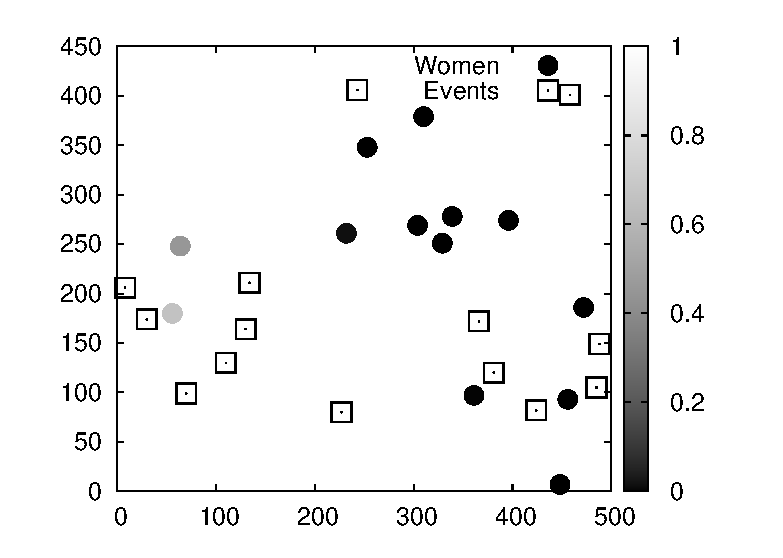
\includegraphics[width=\linewidth,clip]{sol.eps}
\caption[図の例]{図の例}
\label{fig:ex}
\end{figure}
\end{verbatimtab}
のように書くと,
\begin{figure}[htbp]
\centering
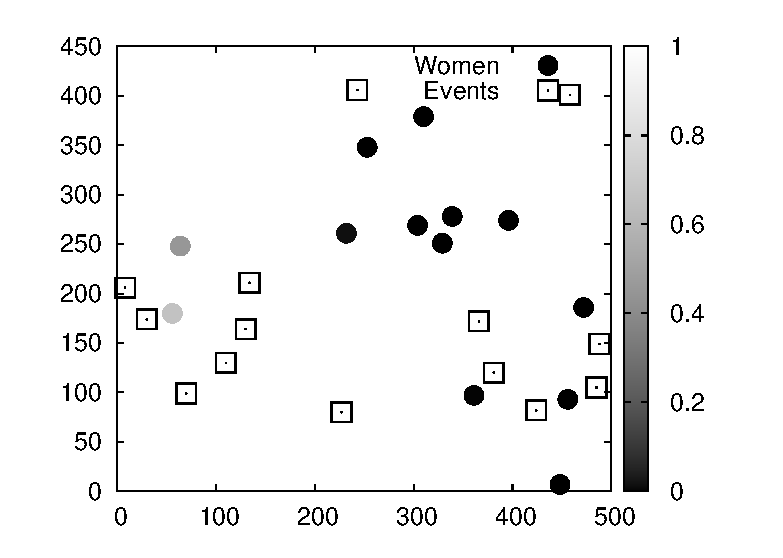
\includegraphics[width=\linewidth, clip]{sol.eps}
\caption[図の例]{図の例}
\label{fig:ex}
\end{figure}
図~\ref{fig:ex}のように表示されます.
全ての図は原則として例示の通りページ幅いっぱいに掲載
(\texttt{includegraphics}命令の\texttt{width}オプションを
\texttt{linewidth}に指定)して下さい.この原則を崩すのは
図がページ高を超えてしまうときに限ります.
図題目は図の下に置くことに注意して下さい.
図の入っているepsファイル(ここでは\texttt{sol.eps})はtexファイルと
同一ディレクトリ内にあるようにして下さい.
尚,図は\LaTeX{}が処理の都合上,
一番良い場所に入れてくれるので,
卒業論文概要書のような分量に制限がある場合を除き,
逆らうべきではありません.
どうしてもという場合だけ\texttt{here.sty}の\text{[H]}を使って下さい.
なお,本研究室では旧来の名残で図ファイル形式にEPSを用いていますが,
現代ではPDFが望ましいです.

図表いずれも,本文中に図表の説明をし,その際に参照機能を用いて下さい.
また,図目次や表目次を確認して,各図表の違いが図題目や表題目で区別がつく
ように適切に題目を設定して下さい.
%
%
%
\section{プログラムソース}\label{sec:multimedia_program}
%
%
%
プログラムソースは本文書付録~\ref{chap:program}にあるように,
全プログラムソースを付録として掲載して下さい.
他人が追跡調査できるように,
\begin{itemize}
\item 不要なコメントや標準出力は削り,
\item インデントや書式を綺麗に
\end{itemize}
して下さい.
具体的な記載方法は,予めtexファイルと同じディレクトリにソースファイル(ここでは仮に\texttt{runge.c}とする)をコピーしておき,
\begin{verbatimtab}
\section*{\texttt{runge1.c}}
\addcontentsline{toc}{section}{\texttt{runge1.c}}
\listinginput{1}{runge1.c}
\end{verbatimtab}
と書くと付録のように表示されます.
なお,PDFや印刷結果の仕上がりを見て,
ページ番号の印字位置よりも右側にプログラムソースが印字されていないよう,
適宜,コンパイルに成功するように改行して下さい.
%
%
%
\section{おわりに}\label{sec:multimedia_summary}
本章では,図表とプログラムソースについて述べました.
まず第\ref{sec:multimedia_table}では表について述べました.
次に第\ref{sec:multimedia_figure}では図について述べました.
最後に第\ref{sec:multimedia_program}ではプログラムソースについて述べまし
た.
%
%
%
\chapter{結論}\label{chap:conclusion}
本文書では,
当研究室で,卒業論文を作成するにあたって,注意すべき事項を記した.
第\ref{chap:first}章では,本文書の背景,目的,構成について
説明した.
第\ref{chap:checkManuscript}章では,指導教員に原稿を校正させることについて
説明した.
第\ref{chap:abst}章では,卒業論文概要書作成について
説明した.
第\ref{chap:thesis}章では,卒業論文作成について
説明した.
第\ref{chap:presen}章では,発表資料作成について
説明した.
第\ref{chap:statement}章では,卒業論文概要書,卒業論文,および発表資料に盛
り込まれる文章について
説明した.
第\ref{chap:math}章では,卒業論文概要書,卒業論文,および発表資料に盛
り込まれる数式について
説明した.
第\ref{chap:experiment}章では,卒業論文概要書,卒業論文,および発表資料に盛
り込まれる数値実験について
説明した.
第\ref{chap:cite}章では,卒業論文概要書,および卒業論文に盛
り込まれる数値実験について
説明した.
第\ref{chap:reference}章では,\LaTeX{}を用いて卒業論文概要書や卒業論文を作
成する際の参照機能を説明した.
第\ref{chap:latex-rule}章では,その他の\LaTeX{}のルールを説明した.
第\ref{chap:multimedia}章では,\LaTeX{}における図表とプログラムソースの取
り扱いについて説明した.
また,付録では,
原稿チェックリスト,過去の卒業研究中間発表会と卒業研究発表における配布資
料を掲載した.
%
%
%
%
%
%
%\chapter{フォントのテスト}
%%
%%
%%
%\section{pifont}
%%
%%
%%
%\ding{"2E}\ding{"21}\Pisymbol{psy}{"A9}
%%
%%
%%
%\section{tascmac}
%%
%%
%%
%\keytop{A}\Return
%%
%%
%%
\begin{thebibliography}{99}
\bibitem{kanzawa}神沢~雄智:精度保証付き数値計算法を用いた非線形方程式の解の数値存在検証法に関する研究, 早稲田大学博士論文 (1998).
\bibitem{mori}森~栗丸:``あじさいの唄'', ビッグコミックオリジナル, No.824, pp.223--230 (2002).
\bibitem{ichigan}一丸:``1年1組~甲斐先生'', ビッグコミックオリジナル, No.824, pp.41--58 (2002).
\end{thebibliography}
\chapter*{感想}
\addcontentsline{toc}{chapter}{感想}\label{chap:feel}
おいしかった.
\chapter*{謝辞}
\addcontentsline{toc}{chapter}{謝辞}\label{chap:ack}
ありがとう.
\appendix
\pagestyle{headings}
\addtocontents{toc}{\protect\diamondeleaders\par}
\chapter{プログラムソース}\label{chap:program}
\section*{\texttt{runge1.c}}
\addcontentsline{toc}{section}{\texttt{runge1.c}}
\listinginput{1}{runge1.c}
\section*{\texttt{runge1.c}}
\addcontentsline{toc}{section}{\texttt{runge1.c}}
\listinginput{1}{runge1.c}
\newpage
\appendix
\pagestyle{headings}
\addtocounter{chapter}{1}
\chapter{原稿チェックリスト}\label{chap:chk_lst}
\noindent
\begin{table}[H]
\caption{原稿チェックリスト}
\centering
\resizebox{0.6\linewidth}{!}{%
\begin{tabular}{p{30zw}|p{3zw}}
\hline
項目&確認欄\\
\hline\hline
流れ図と原稿は合致するか&\\
\hline
「〜だが」や「しかし」などの接続詞は続けて現れていないか&\\
\hline
1文の長さは長すぎないか&\\
\hline
読点は少なすぎないか&\\
\hline
「〜なので」,「よって」.「したがって」などの接続詞が使い分けられているか&\\
\hline
漢字にすべき語をひらがなにしていないか&\\
\hline
文章中に丸括弧を用いて注意書きに相当する内容を盛り込んでいないか&\\
\hline
文章の箇条書きを極力避けたか&\\
\hline
全ての文章に主語はあるか&\\
\hline
全ての文章の主語と述語は合致しているか&\\
\hline
必要な章を全て盛り込んでいるか&\\
\hline
各章の順は指定通りか&\\
\hline
各章の題目は指定通りか&\\
\hline
全ての記号は定義済みか&\\
\hline
重要な定義・定理・例などに対して
\LaTeX
の環境を使用しているか&\\
\hline
表・図には題目・番号が記され,本文中で引用・説明されているか&\\
\hline
数式に数式番号が入っているか&\\
\hline
文章中の数式(1記号のみの場合は除く)はdisplaystyleで書かれているか&\\
\hline
数式はすべて数式モードか&\\
\hline
$sin$などは$\sin$となっているか&\\
\hline
括弧の大きさは適当か&\\
\hline
微分・積分の$\mbox{d}$など数式中のRoman体を使用しているか&\\
\hline
人名は原語で書かれ,頭文字のみ大文字でその他は小文字であるか&\\
\hline
英数字は半角で書かれているか&\\
\hline
参考文献は全て掲載されているか&\\
\hline
参考文献は引用されているか&\\
\hline
参考文献の書式は指定通りか&\\
\hline
\end{tabular}}
\end{table}
%
%
%
\chapter{過去の中間発表会関連配布資料}\label{chap:chukan}
%
%
%
\begin{figure}[htbp]
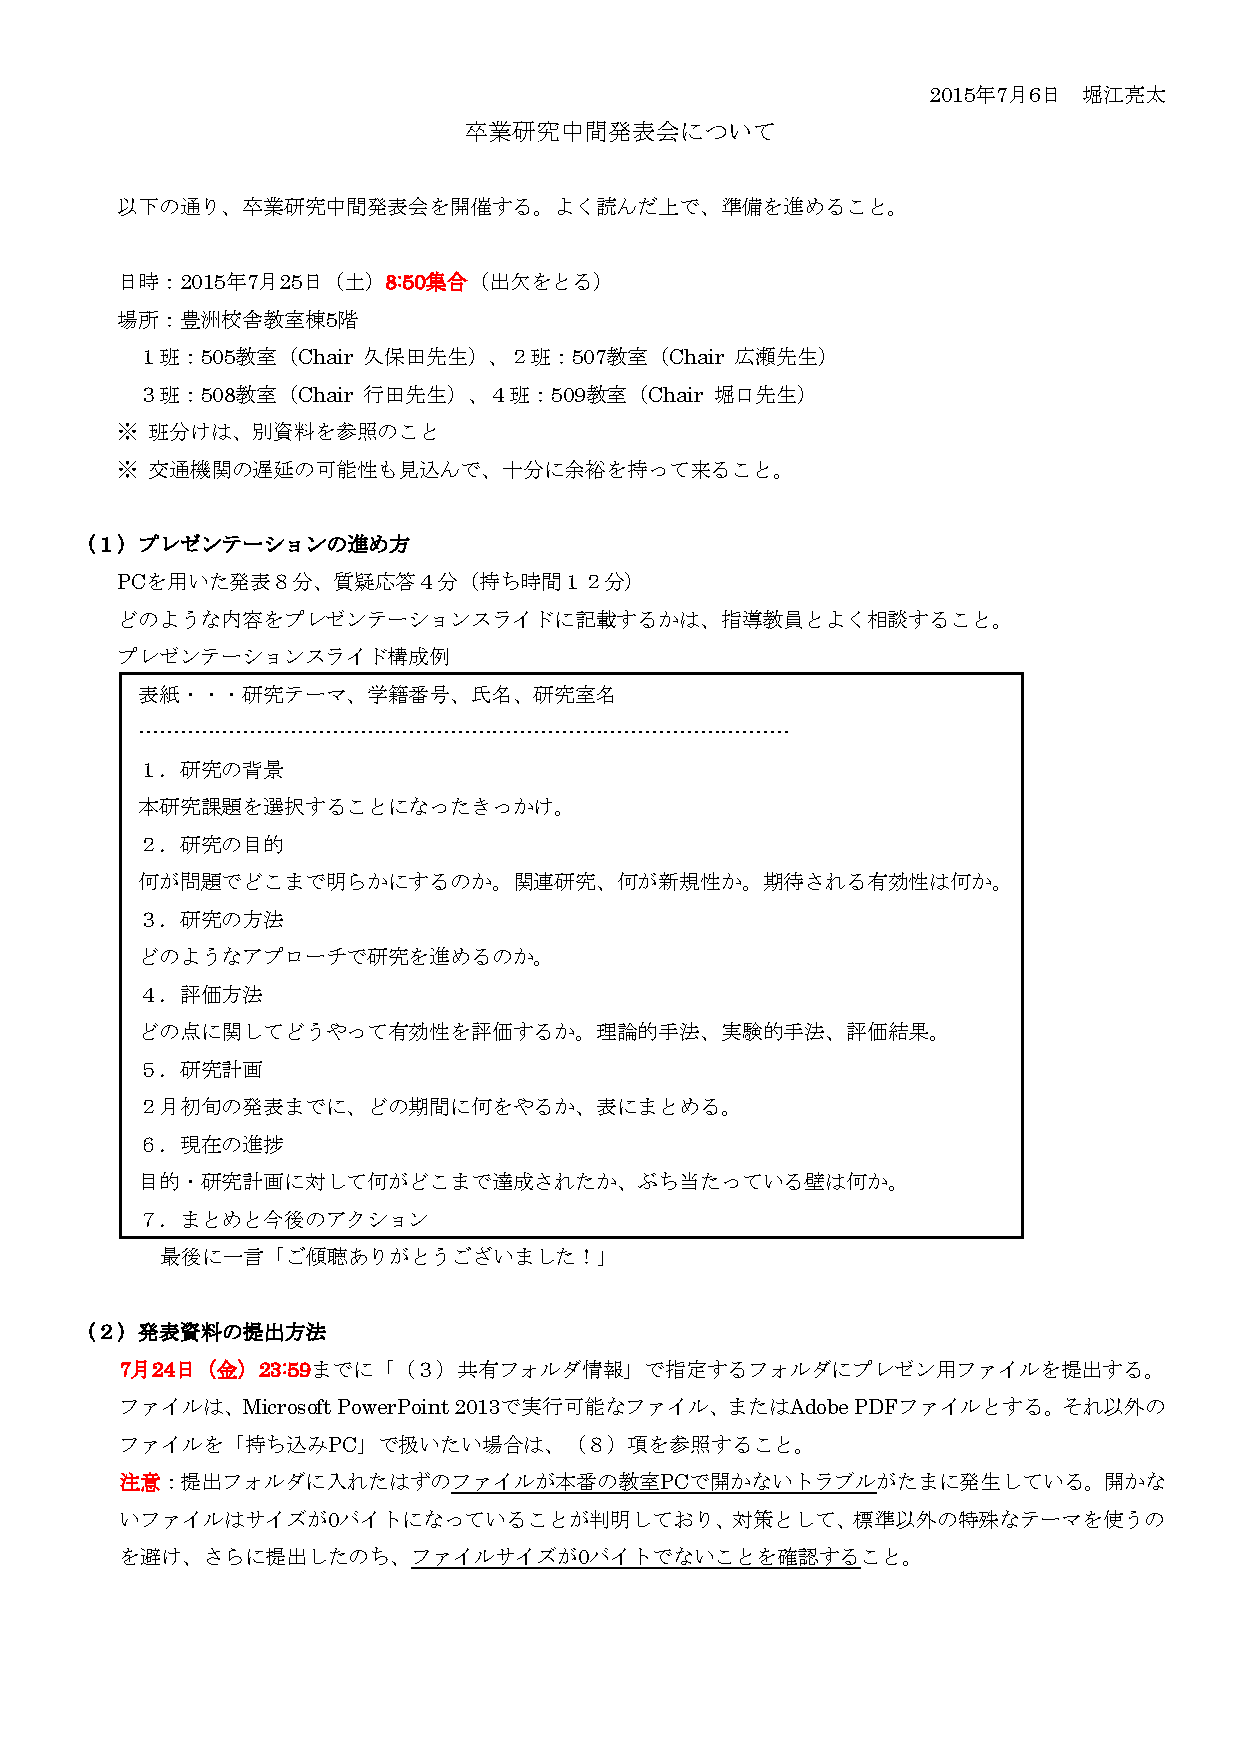
\includegraphics[width=0.65\linewidth]{chukanAnnounce.pdf}
\caption{2015年度卒業研究中間発表会案内文書}
\label{fig:chukanAnnounce}
\end{figure}
\begin{figure}[htbp]
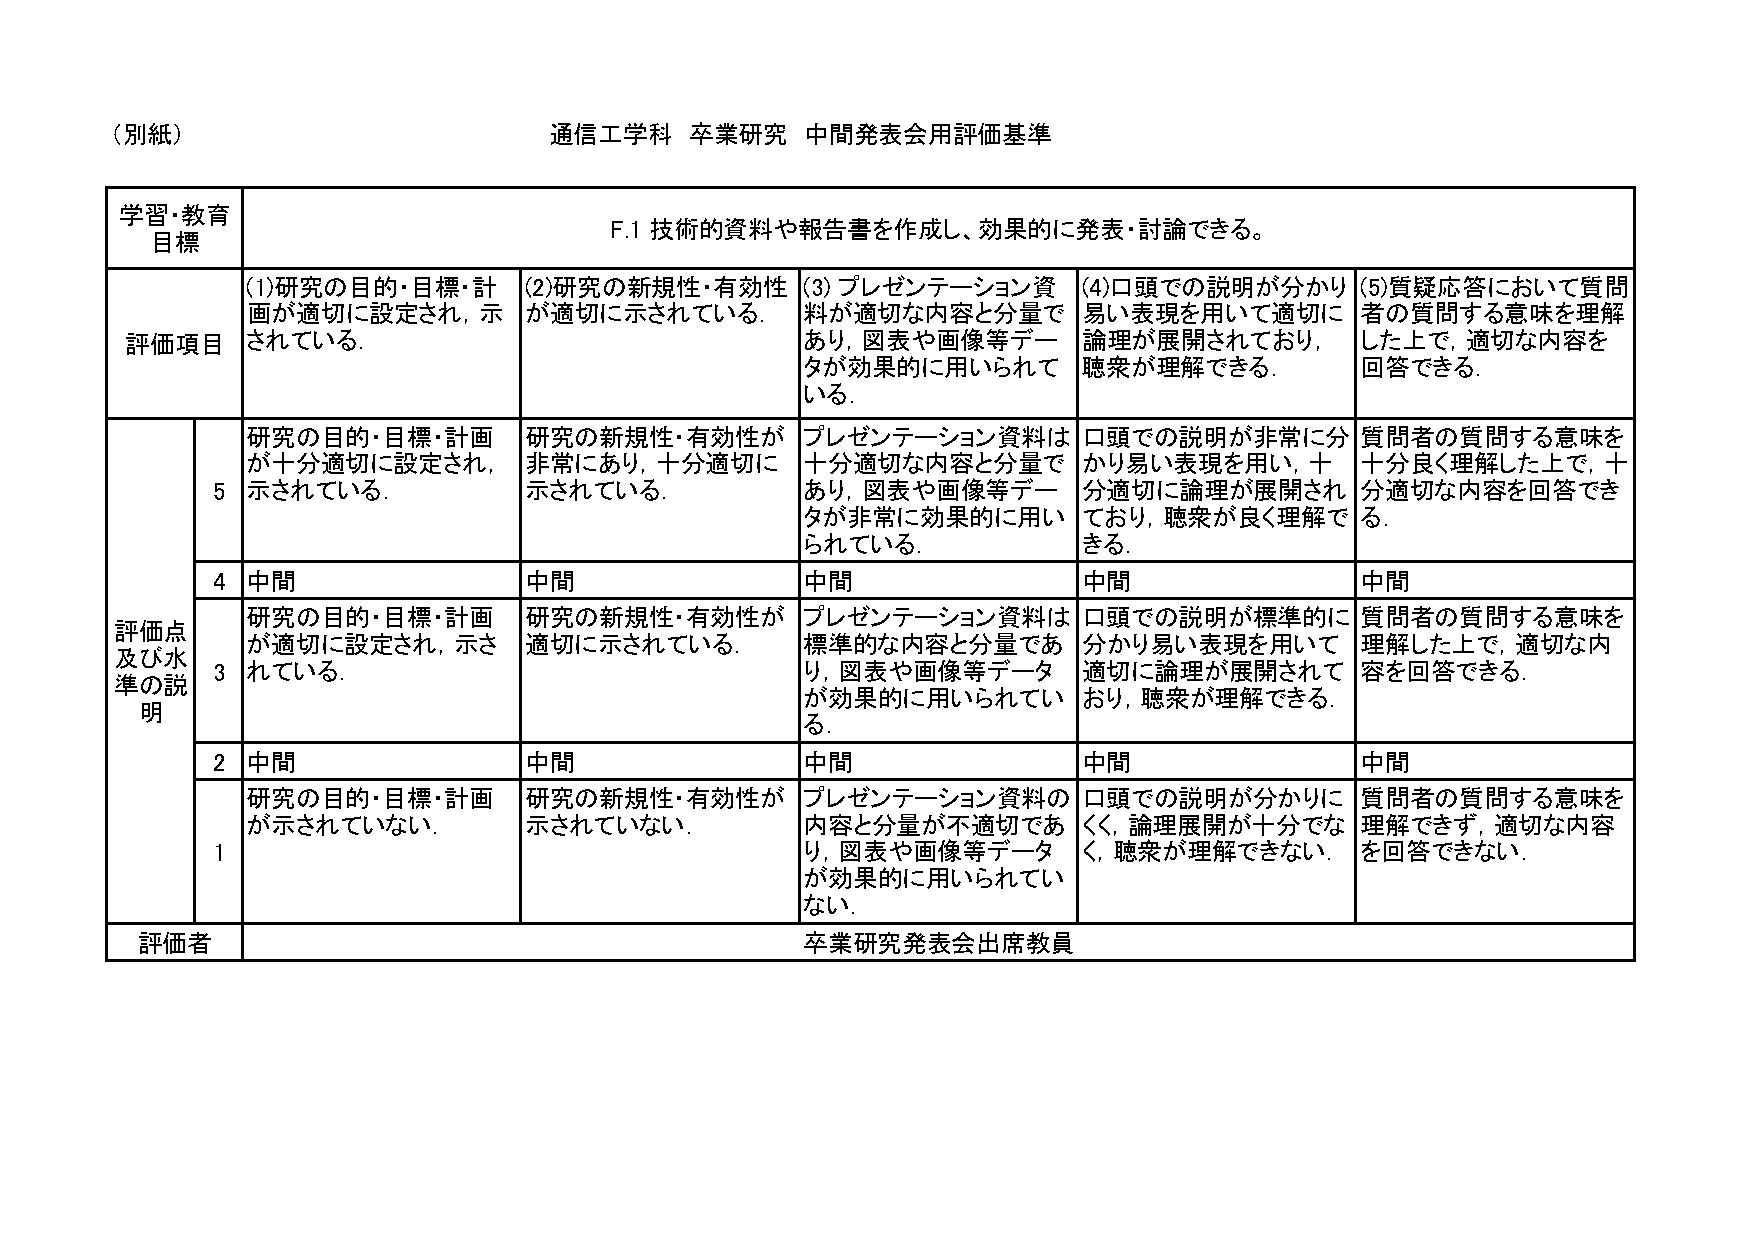
\includegraphics[width=\linewidth]{chukanLevel.pdf}
\caption{2015年度卒業研究中間発表会評価基準}
\label{fig:chukanLevel}
\end{figure}
%
%
%
\chapter{過去の卒業研究発表会関連配布資料}\label{chap:last}
%
%
%
\noindent
\begin{figure}[htbp]
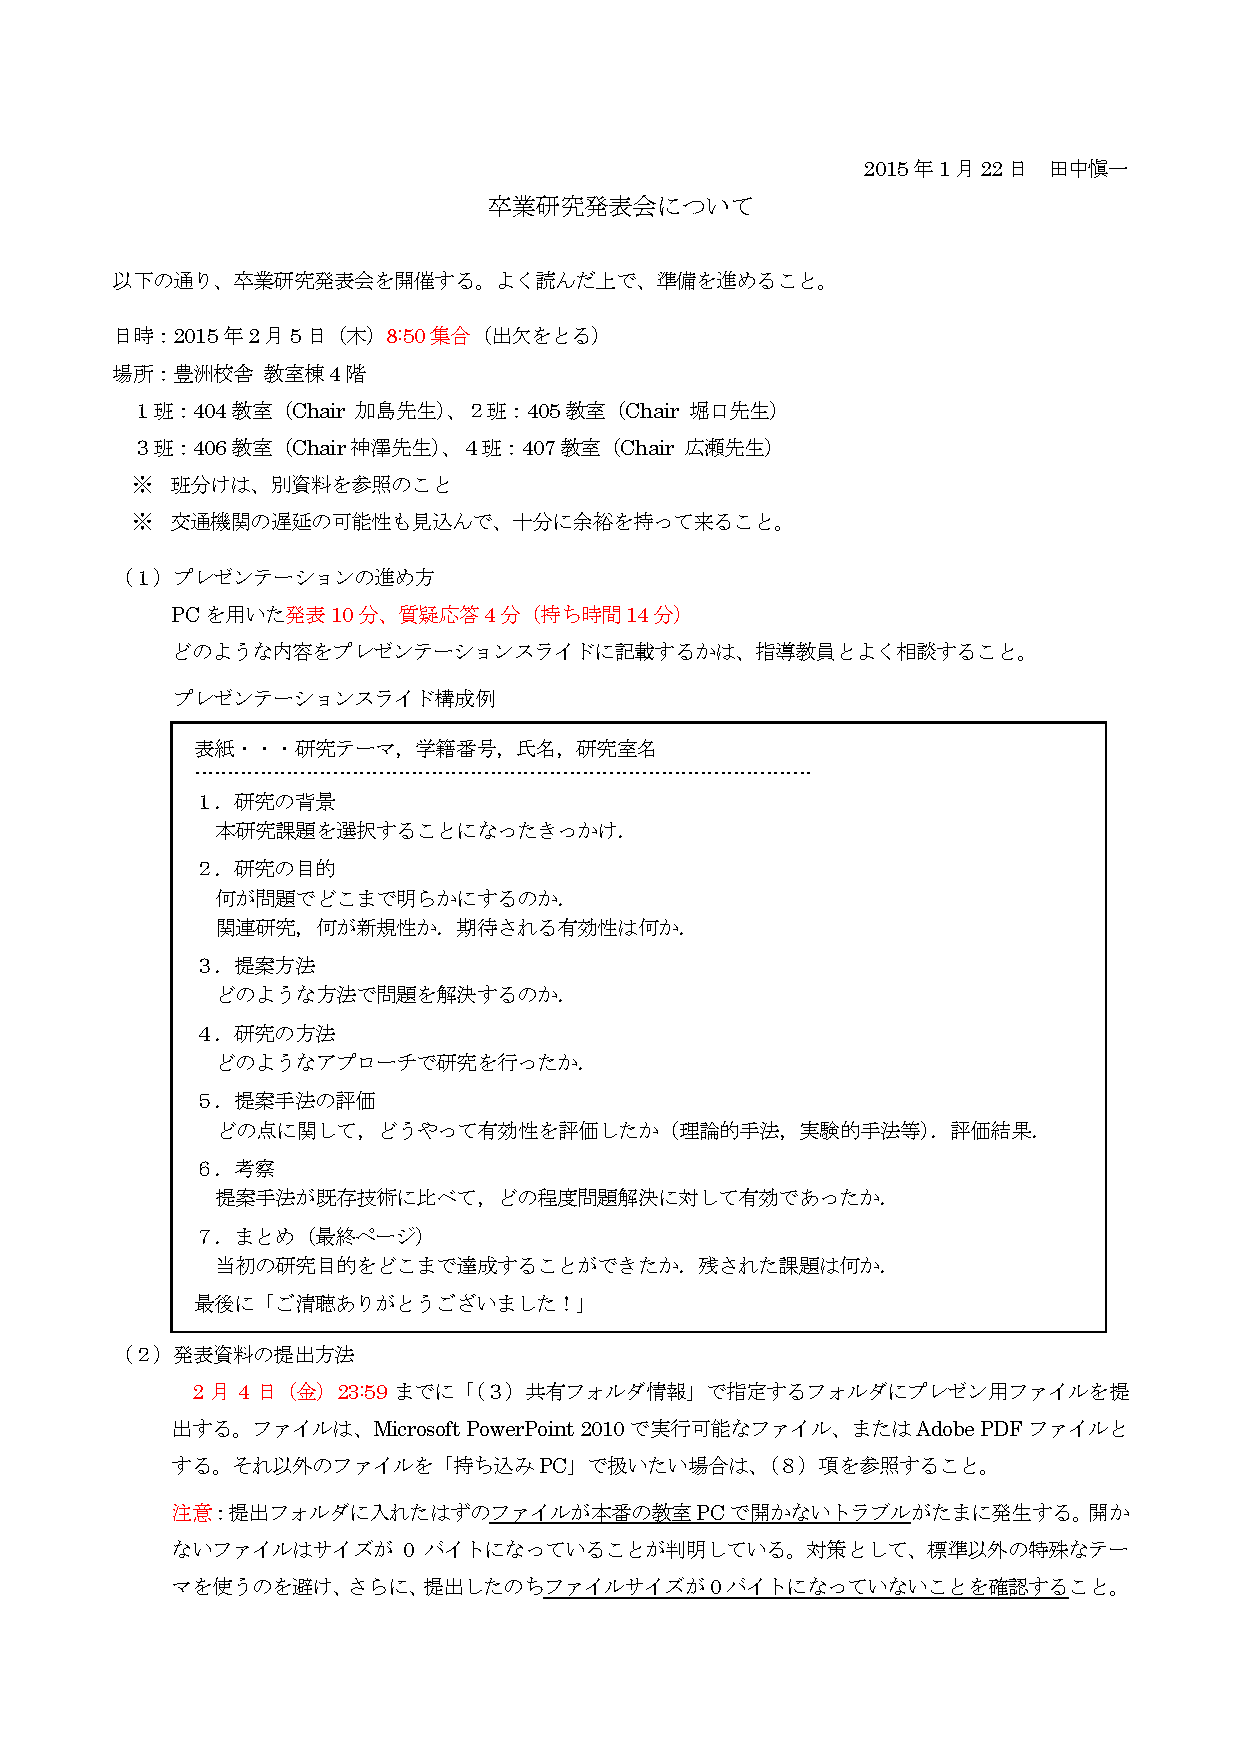
\includegraphics[width=0.65\linewidth]{presenAnnounce1.pdf}
\caption{2014年度卒業研究発表会案内文書}
\label{fig:presenAnnounce1}
\end{figure}
\begin{figure}[htbp]
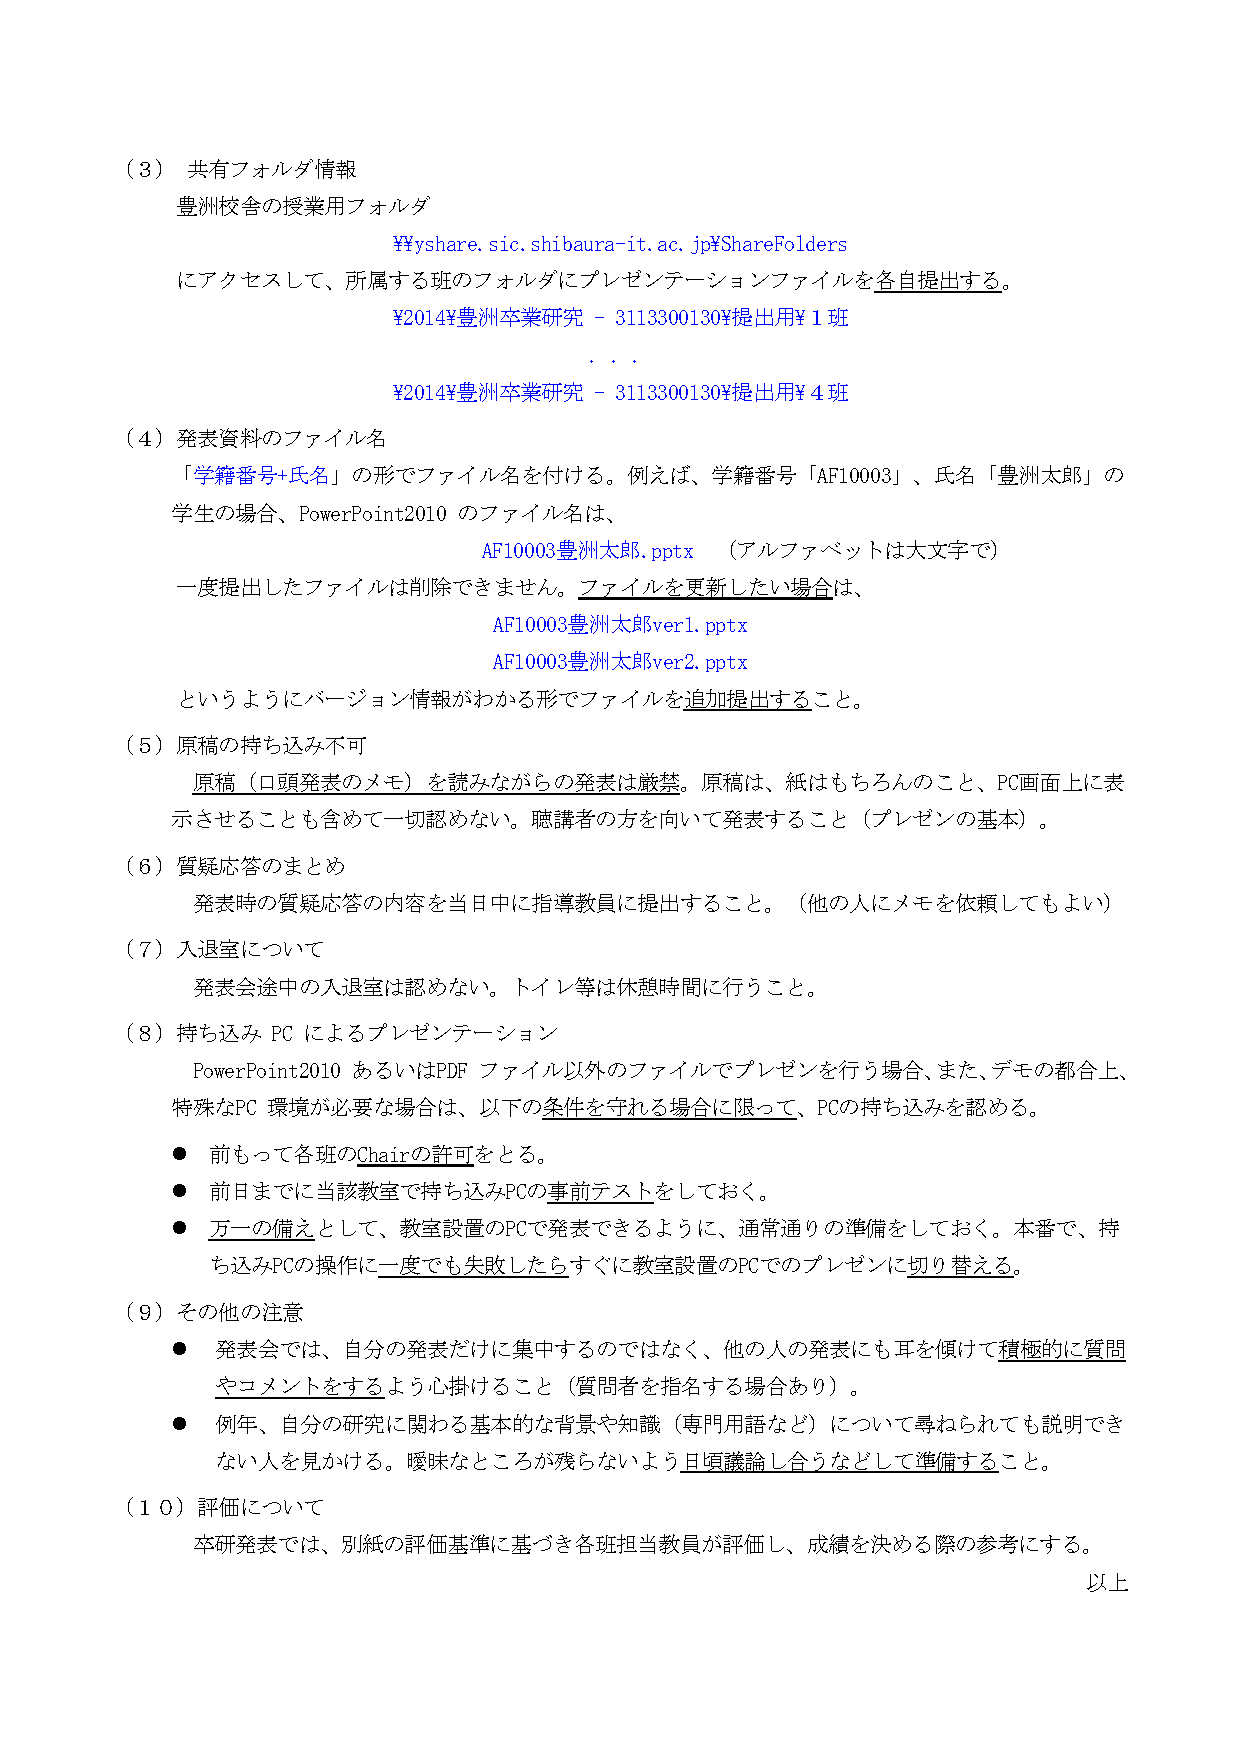
\includegraphics[width=0.8\linewidth]{presenAnnounce2.pdf}
\caption{2014年度卒業研究発表会案内文書の続き}
\label{fig:presenAnnounce2}
\end{figure}
\begin{figure}[htbp]
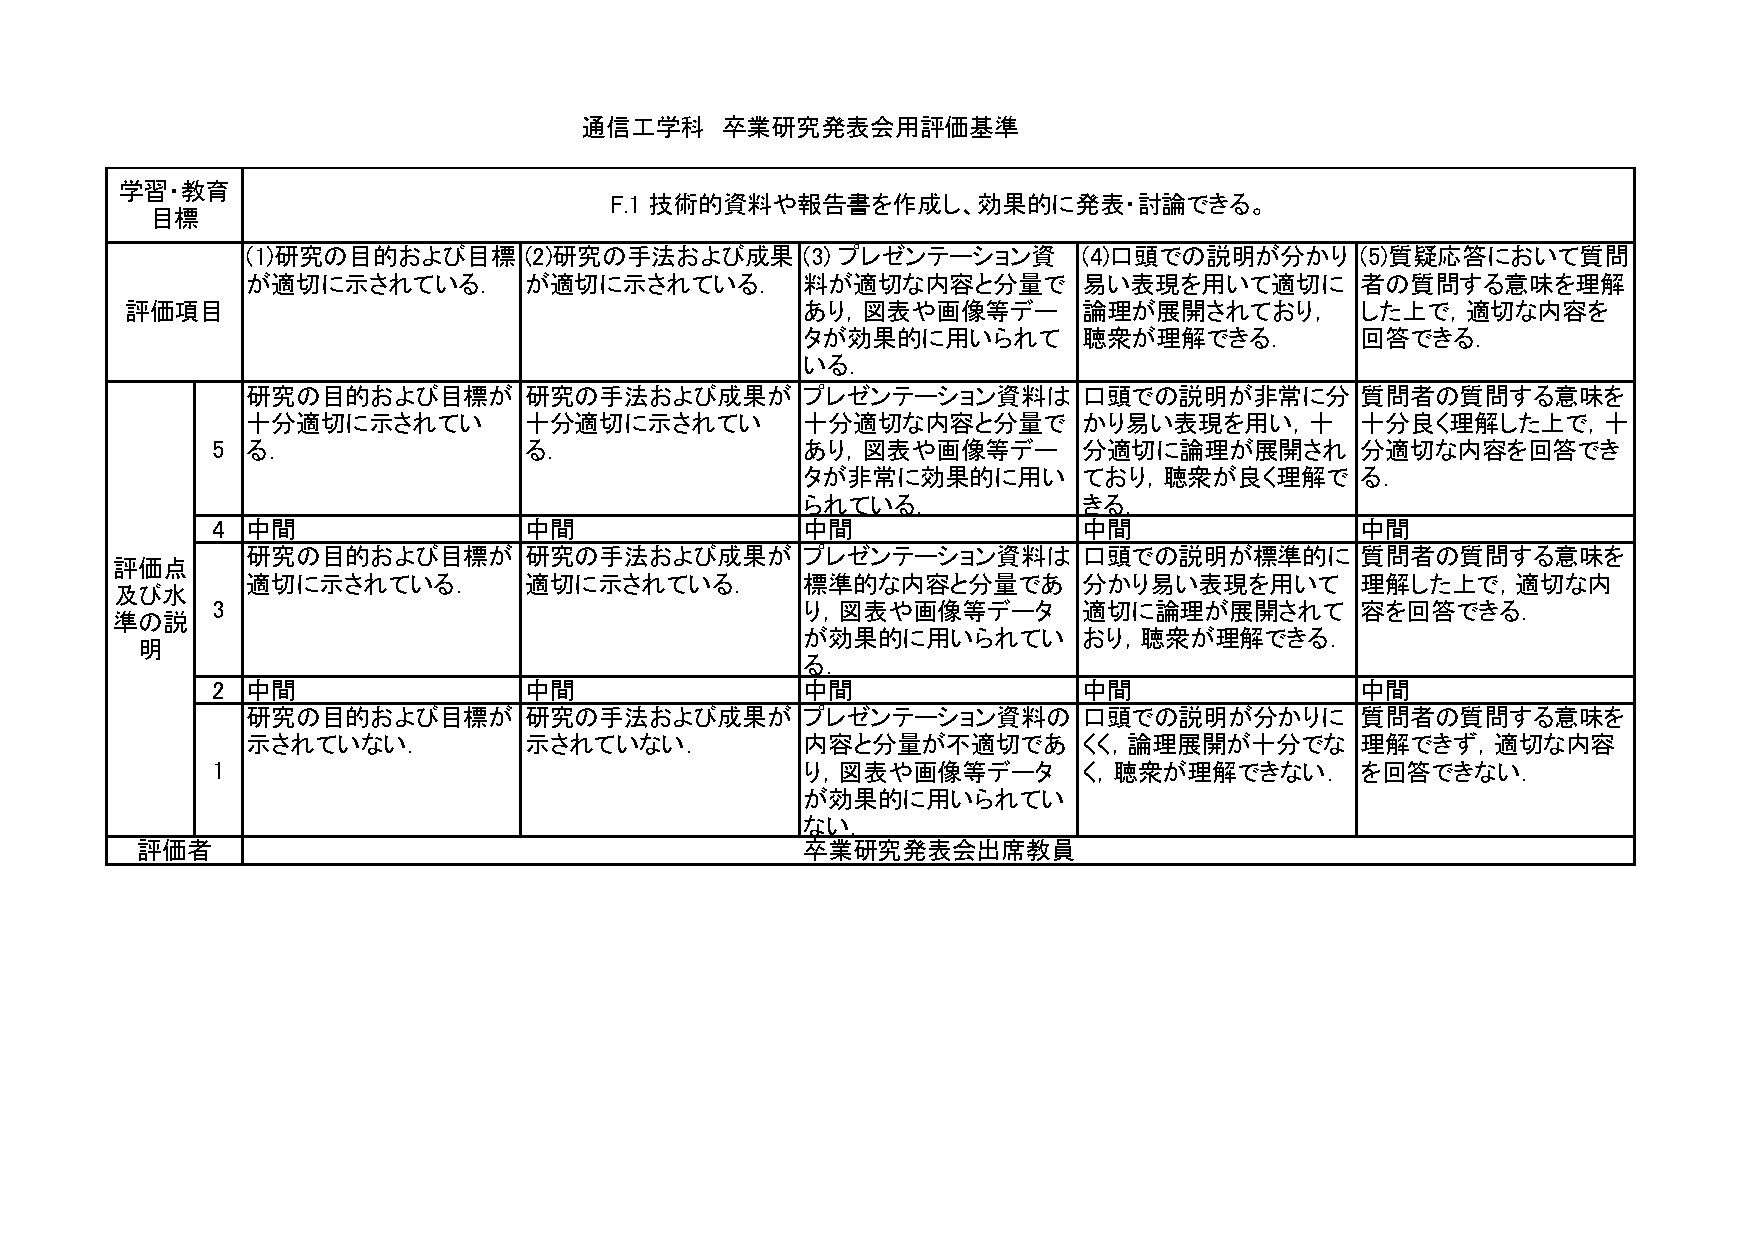
\includegraphics[width=\linewidth]{presenLevel.pdf}
\caption{2014年度卒業研究発表会評価基準}
\label{fig:presenLevel}
\end{figure}
\end{document}

